\chapter{Calibration Methods}\label{chap:calibration}
In order to use a qubit and in particular if we want to simulate said qubit, we need to learn the most important parameters. In this section, we will go through the different methods used for calibrating a qubit and the connected resonator in order to have a useful qubit along with the possibilities of simulating the system.


\section{Qubit Calibration}
Before using a qubit, it will be necessary to characterize it to the best of our ability, in this section, we will go over the standard methods for characterizing the necessary qubit and resonator properties. In this thesis experiments and simulations were done on a Transmon system.

\subsection{Spectroscopy}
To drive the qubit and simulate the most important quantity is to extract the qubit frequency. This is done by doing qubit spectroscopy, where the qubit is driven out by a pulse of a given frequency and then read out. At the qubit frequency, we will expect the qubit to get excited with a higher probability. In addition to the qubit frequency $f_{01}$ the anharmonicity is all of interest, if we want to model the qubit as a 3 level-system. Since the design of the transmon gives a negative anharmonicty \todo{Reference transmon sections}, we can extend the qubit spectroscopy, to also look for a transition from $\ket{0}\to \ket{2}$. This can be done either with $f_{02}$ or by absorbing two photons of $f_{02} / 2$. This peak will be at $f_{01} - \alpha / 2$ \todo{Be consistent in sign of $\alpha$}. 
\begin{figure*}[t]
    \caption{Qubit spectroscopy for the $f_{01}$ transition frequency to the left. On the right is an extended scan where another peak is seen, this is the $f_{02}/2$ where two photons are absorbed to go from $ 0 \to 2$. The fits are Lorentzian for one peak and the sum of two Lorenzian for the two peak spectroscopy. }
    \begin{minipage}{0.50\linewidth}
        \centering
        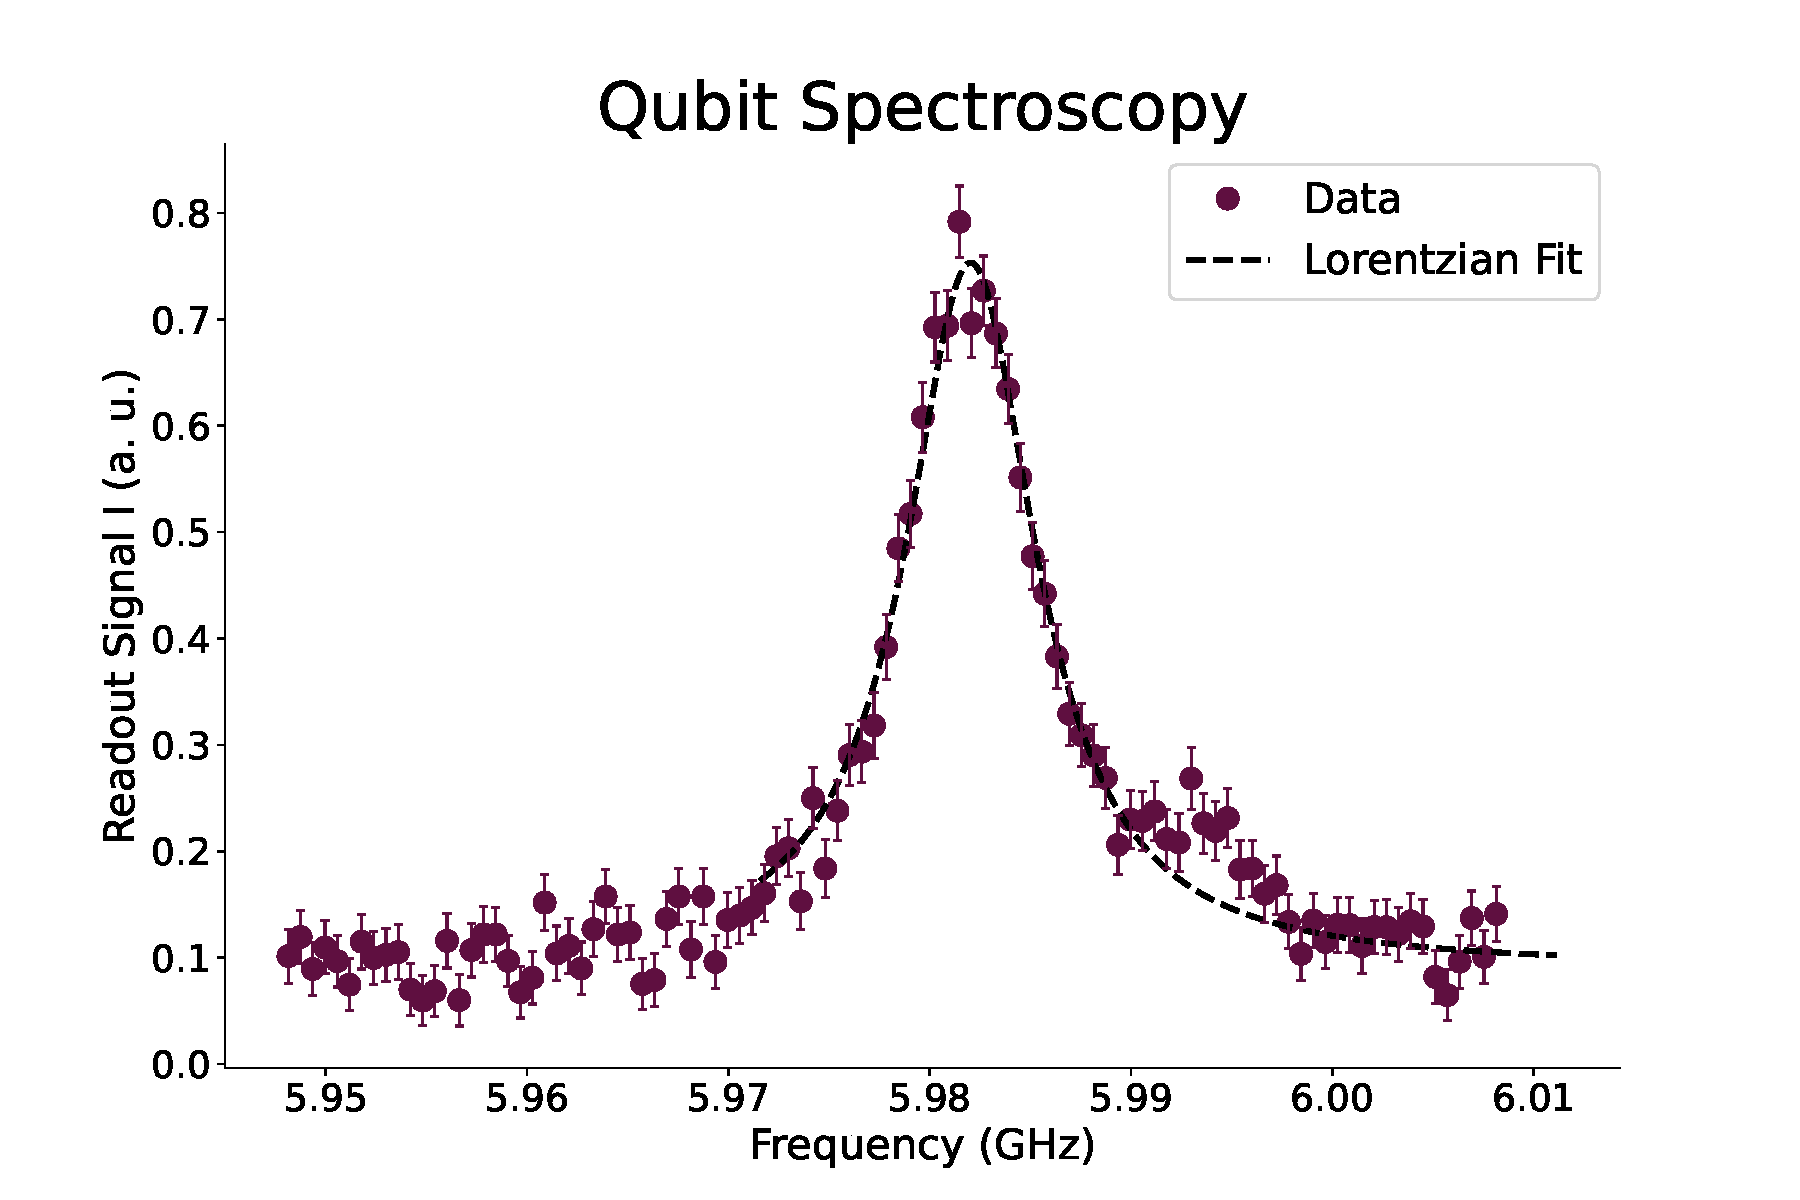
\includegraphics[width=1.0\linewidth]{Calibrations/Figures/Qubit Spectroscopy.pdf} % first figure itself
    \end{minipage}
    \begin{minipage}{0.50\linewidth}
        \centering
        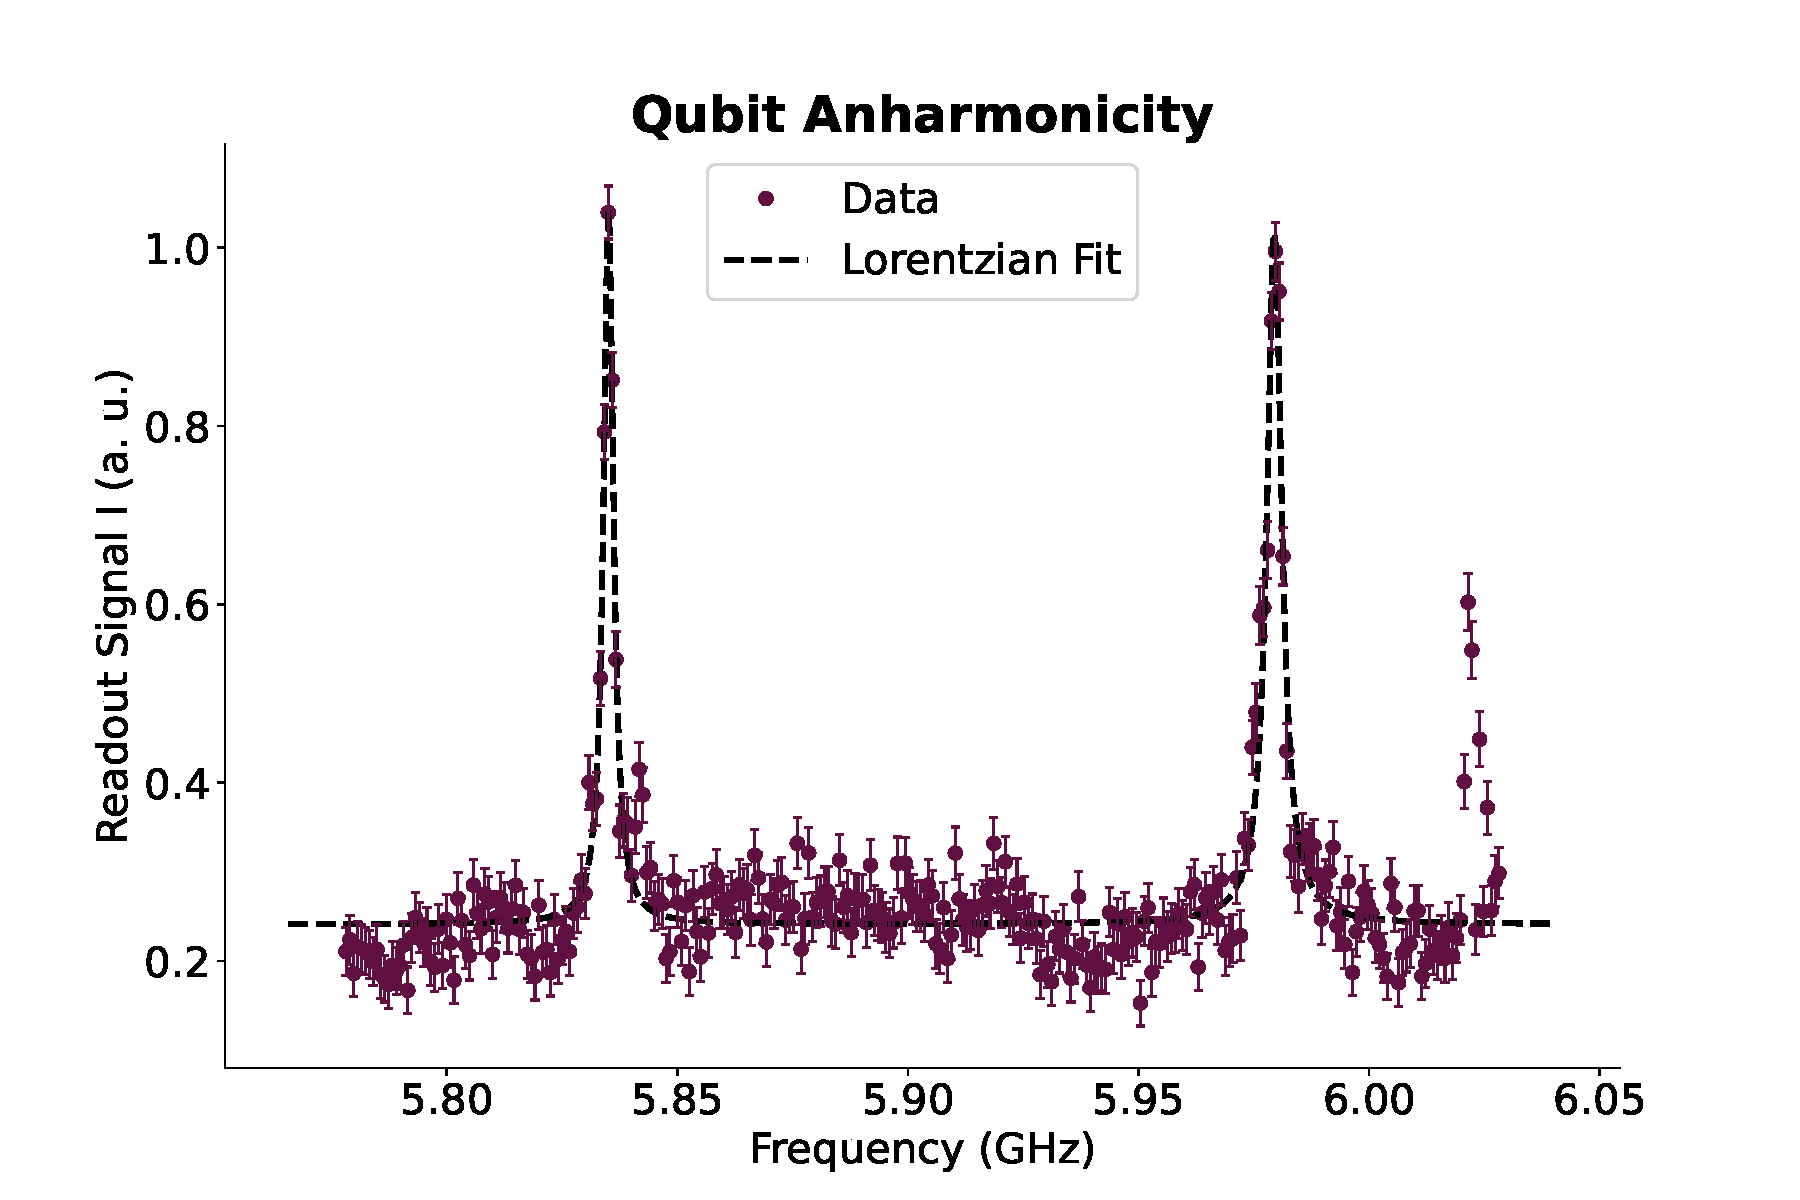
\includegraphics[width=1.0\linewidth]{Calibrations/Figures/Qubit Anharmonicity.pdf} % second figure itself
    \end{minipage}
    \label{fig:qubit_spectroscopy}
\end{figure*}

The two scans for the qubit frequency and half of the $f_{02}$ can be seen in figure \ref{fig:qubit_spectroscopy} along with Lorentzian fits for 1 and 2 peaks respectively. From the fit, we extract:
\begin{equation}
    f_{01} = (5.98203 \pm 0.00008) \text{ GHz}
\end{equation}
And the anharmonicity is calculated as:
\begin{equation}
    \alpha = f_{02} - 2f_{01} = (-288.81 \pm 0.15) \text{ MHz}
\end{equation}


\subsection{Rabi}
In section \ref{sec:how_to_make_gates}, we saw how one can make an x- and y-gates. By driving at the qubit frequency and in the $I$ quadrature found in the previous section, the form of the effective Hamiltonian will simply be of the form $H_{eff} = \Omega s_(t) \sigma_x$, which gives the time evolution operator:
\begin{equation}
    \unitary(t) = \exp\left(-i\int_0^t dt' \Omega s(t') \sigma_x \right)
\end{equation}
\begin{marginfigure}[5 cm]
    \centering
    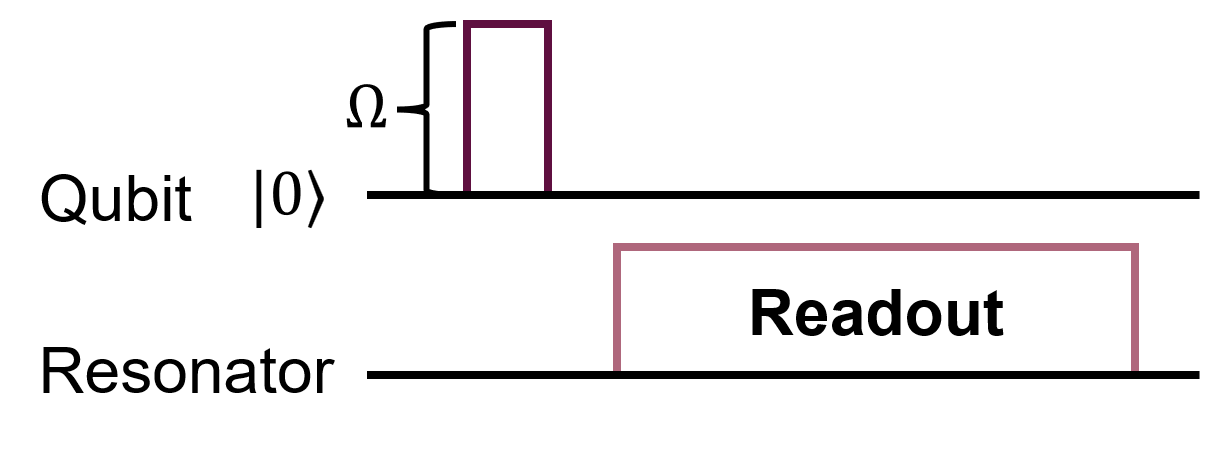
\includegraphics[]{Figs/circuits/rabi.png}
    \caption{The pulse sequence to determine the rabi amplitude. By varying the amplitude depicted with $\epsilon$ and reading out the signal, the optimal $\epsilon$ can be determined.}
    \label{fig:enter-label}
\end{marginfigure}
So to get an x-gate, we can decide on a given envelope function $s(t)$, such that $S = \int_0^t  dt' s(t')$. Thus the dynamics can be altered by simply adjusting the amplitude. If we do a simple experiment, where we initialize the qubit in state $\ket{0}$ and do a pulse with a frequency $\omega_d = \omega_q$ and amplitude $\Omega$ before reading it out. We will see oscillations depending on the area of the curve. Each top will correspond to a $\pi +n2\pi$ rotation around the $x$-axis, where the qubit will be in $\ket{1}$ and the bottoms will be at $2\pi n$ rotations, where we are back at zero. Thus we can fit a cosine curve and by determining its frequency, we can pick the amplitude yielding us a $\pi$ rotation. To go from this pulse to a $\pi/2$ rotation, we can simply pick half of the $X_{\pi}$ amplitude.

\begin{figure}
    \centering
    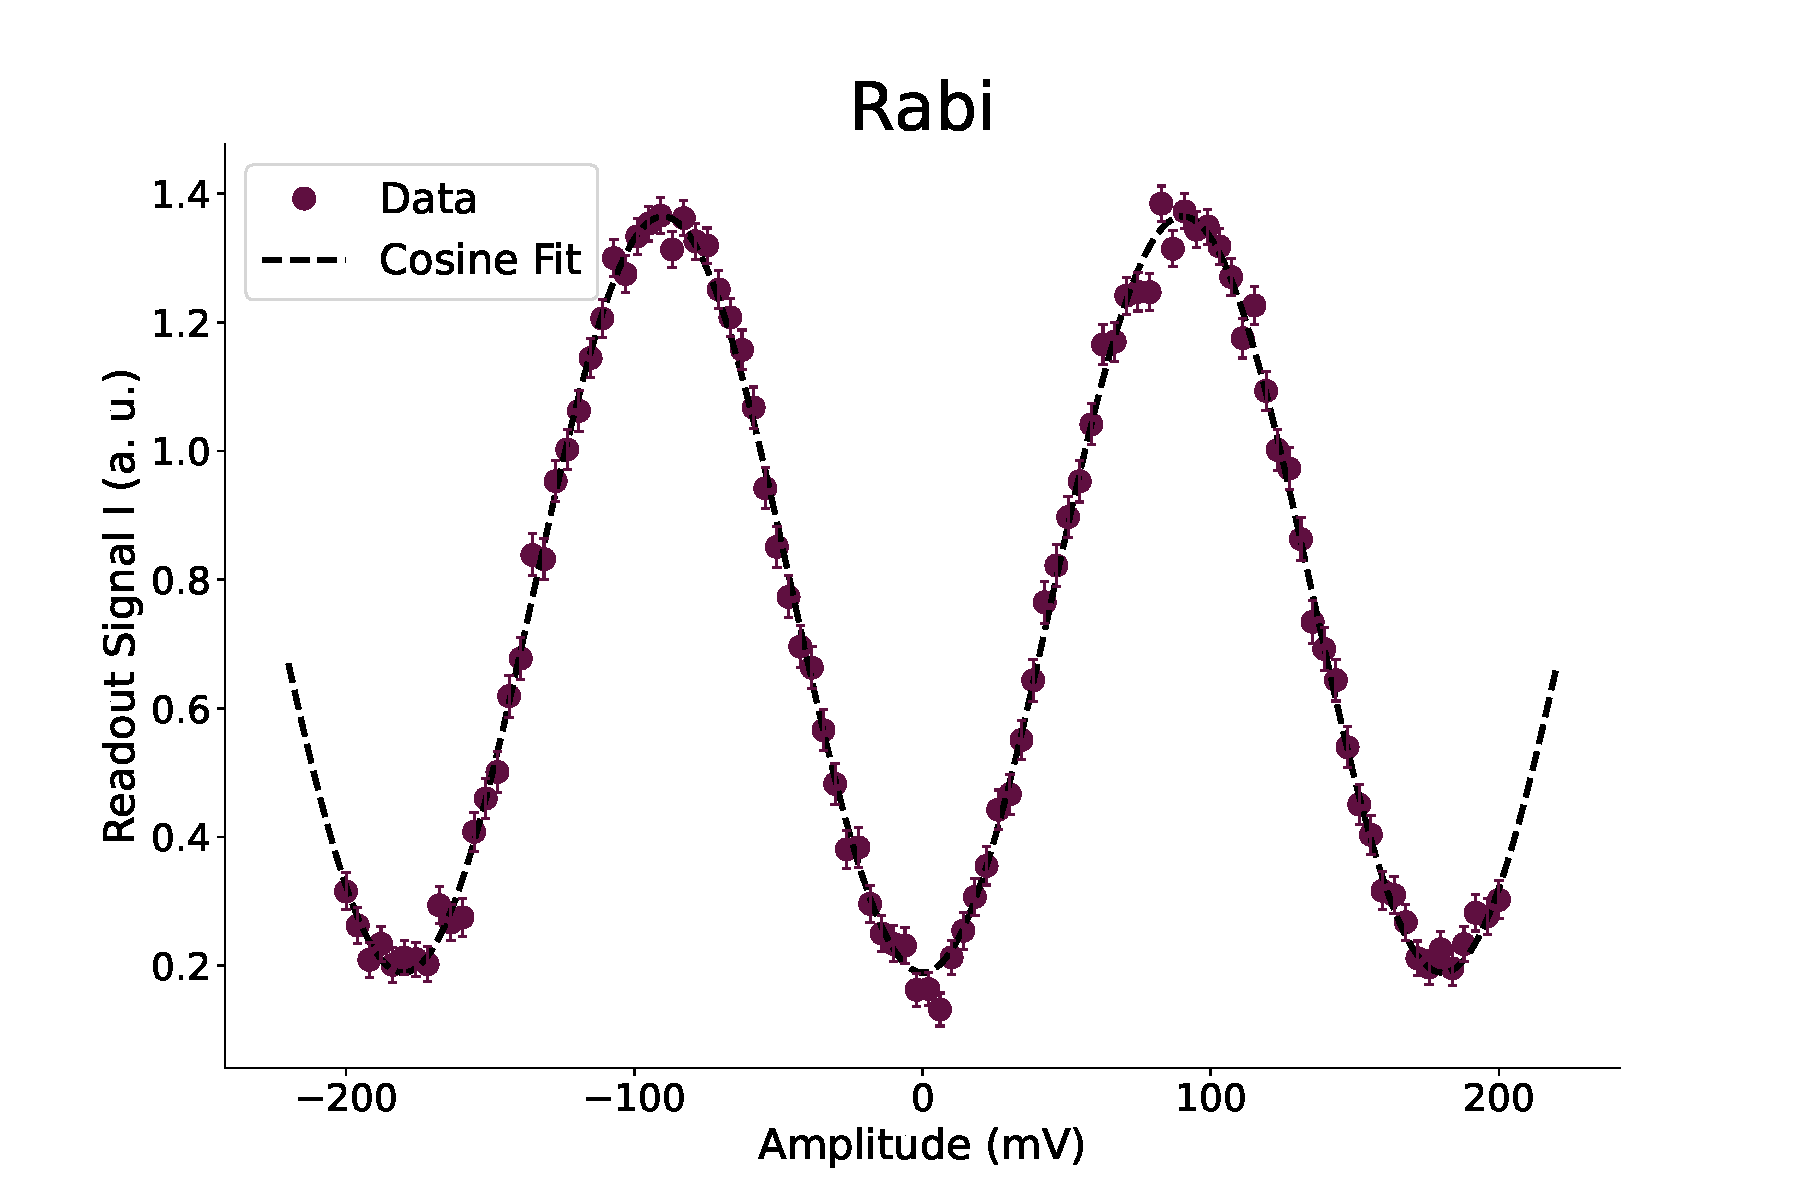
\includegraphics{Calibrations/Figures/Rabi.pdf}
    \caption{The outcome of a Rabi experiment. By varying the amplitude we get a cosine like behaviour which can be fitted to determine the top of the first wave. The curve is fitted with a function of the type: $y = A \cos(2 \pi x f + \phi) + b$ where x is the amplitude, y the outcome and $A, f, \phi$ and $B$ are the fitted parameters.}
    \label{fig:calibration_rabi}
\end{figure}
\noindent
In reality, the pulse also includes a more sophisticated envelope function which supresses the transition from $\ket{0}\to\ket{2}$ by applying the DRAG scheme \cite{motzoi_simple_2009}. And the fidelity of the pulses can be determined by using a randomized benchmarking ... \todo{Do we want to comment on this? } While these parameters are important to make an X-gate in experiement in order to initialize in $\ket{1}$. In simulation, this calibration is not necessary, because we can just apply the pauli x operator to the qubit. 

By doing a randomized bench marking strategy, one can approximate the average gate fidelity. This was done to find average gate fidelity of $F_{\text{gate}} = 0.9913 \pm 0.0003$. This could be included in our in the state initialization error, but the infidelity contribution is much lower than the other contributions initialization fidelity, so we will assume the intilization to have a symmetric error.


\subsection{Decay Calibration}\label{sec:calibration_t1}
\begin{marginfigure}
    \centering
    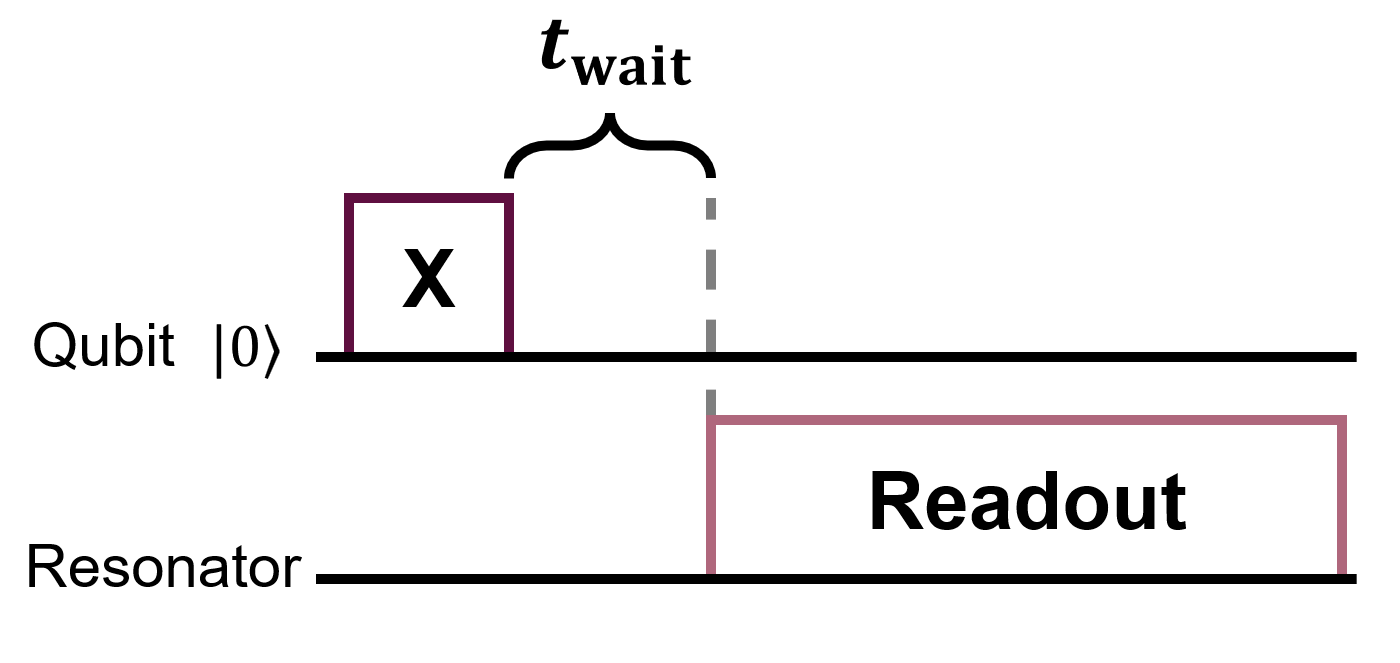
\includegraphics[]{Figs/circuits/t1.png}
    \caption{Caption}
    \label{fig:enter-label}
\end{marginfigure}

From section \ref{sec:theory_t1}, we see that the characteristic logitudinal decay time, $T_1$ can be described by the $\rho_{00}(t)$ and $\rho_{11}(t)$. For this experiment, we will initialize the qubit in state $\ket{1}$ since this is the furthers from steady state. By waiting a time $t_{\text{wait}}$ before reading out the signal and repeating the experiment a certain amounts of time, we can approximate  $\rho_{00}(t)$ and $\rho_{11}(t)$ by taking the average at each time step. Now plotting the occupation as a function om time, we will opbatin a decaying function going toward the steady state. The exponential coefficient of this decay is the $T_1$ time. 


Doing the experiement on our qubit, we obtain the results displayed in figure \ref{fig:calibration_T_1_decay}. The exponential fit gives the value for $T_1$:
\begin{equation}
    T_1 = (4.30 \pm 0.12) \text{ µs}
\end{equation}

\begin{figure}
    \centering
    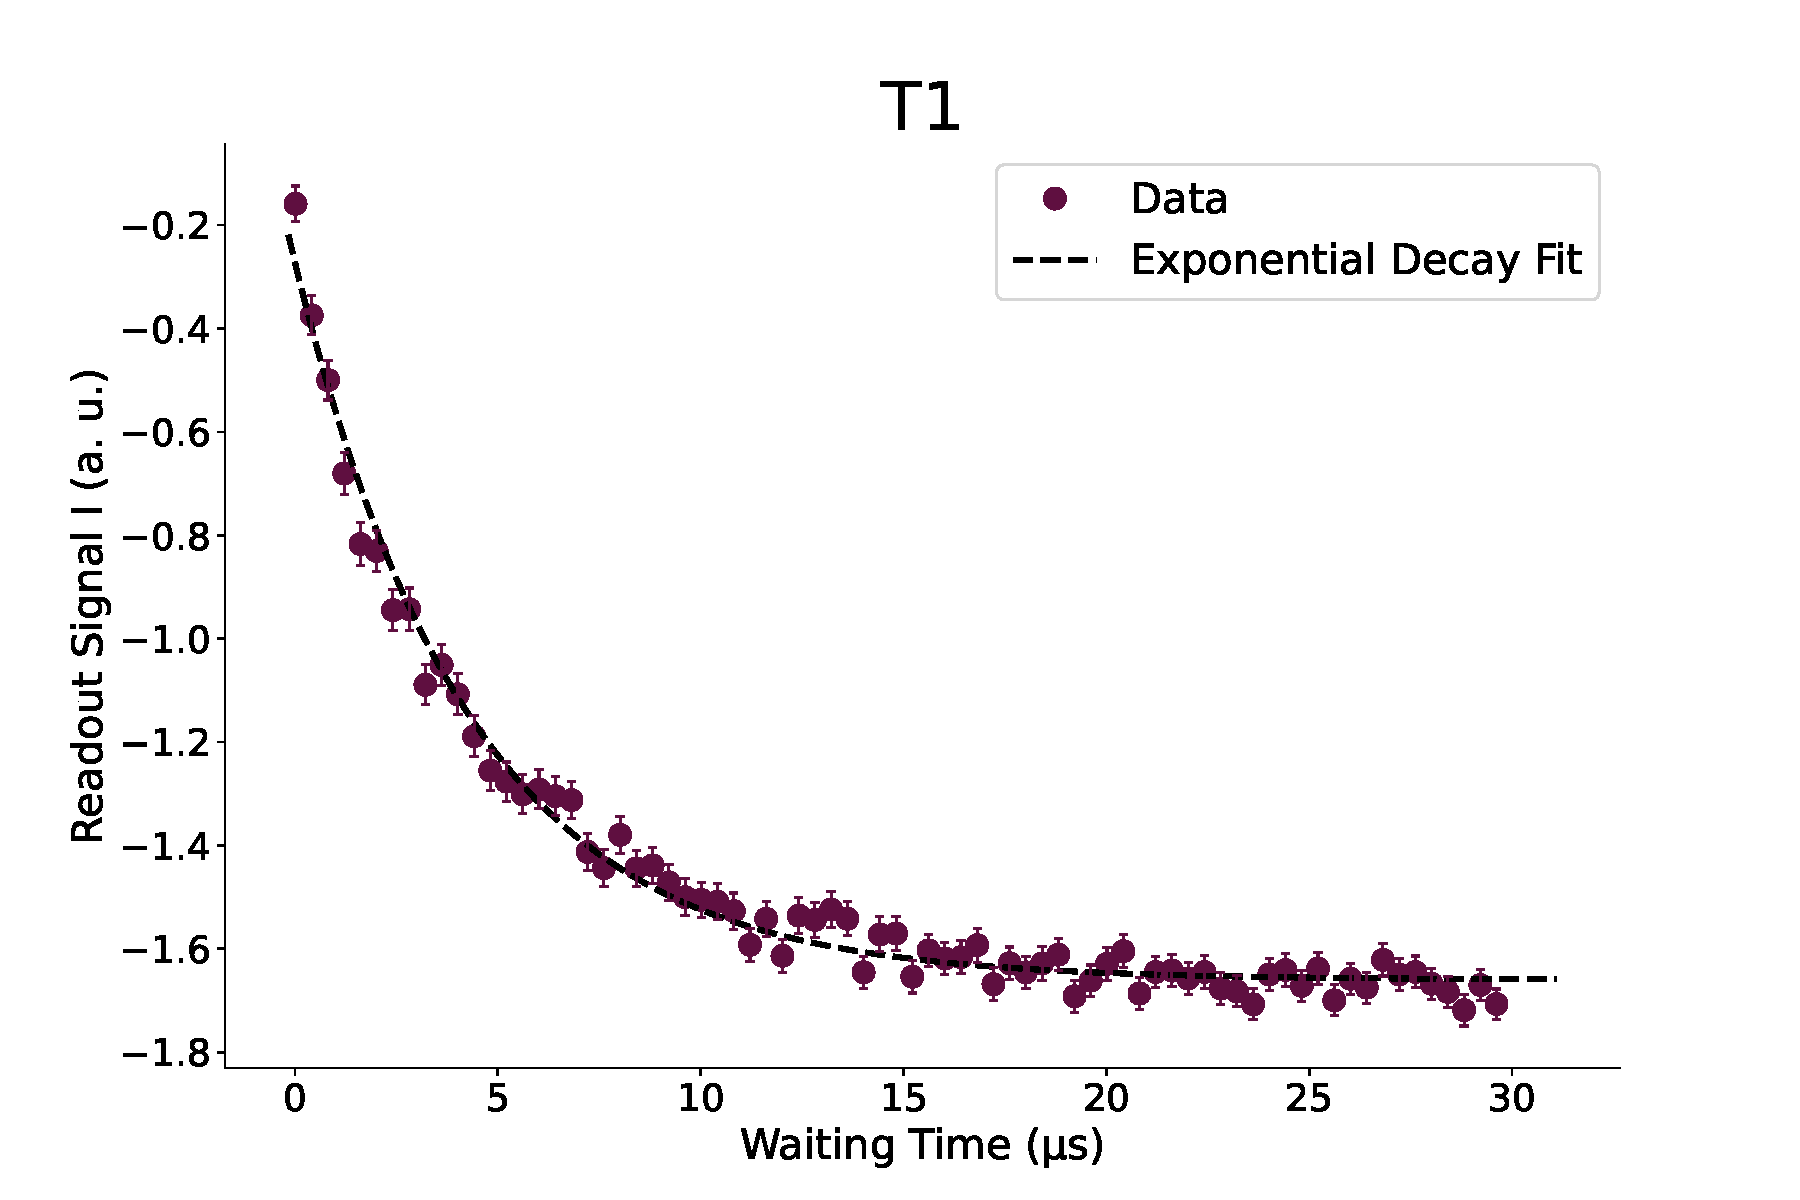
\includegraphics[]{Calibrations/Figures/T1.pdf}
    \caption{Data from an experiment determining the characteristic $T_1$ decay time. The fit is an exponential decay given by: $y = A e^{-t / T_1} + b$ where $t$ is the waiting time, $y$ is the outcome of the experiment and $A, b$ and $T_1$ are fit parameters.}
    \label{fig:calibration_T_1_decay}
\end{figure}

An important note on the $T_1$ is that it varies a lot over a time interval. For this reason ... \todo{Redo Jacobs Figure into my own style.}



\begin{marginfigure}[-5 cm]
    \centering
    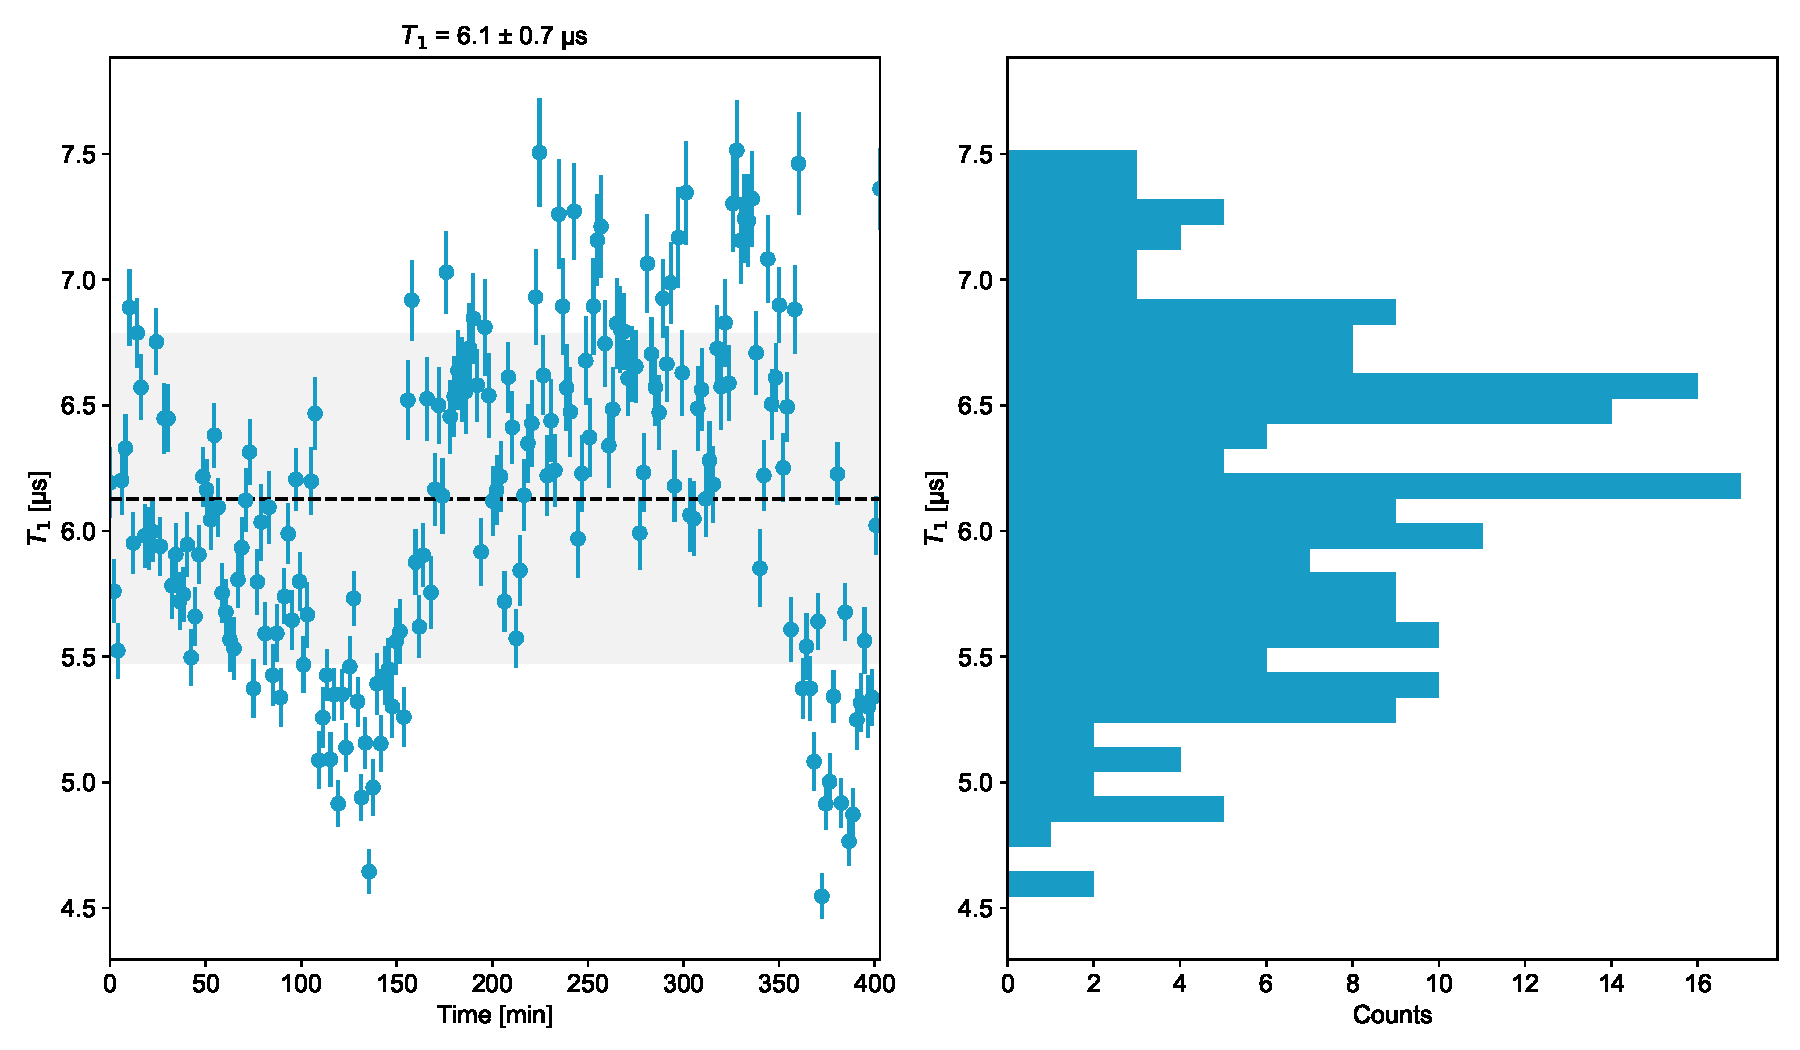
\includegraphics[]{Calibrations/Figures/T1_over_time.pdf}
    \caption{How $T_1$ can change over a few hours}
    \label{fig:changing_t1}
\end{marginfigure}

\subsection{Dephasing Calibration}
\begin{marginfigure}
    \centering
    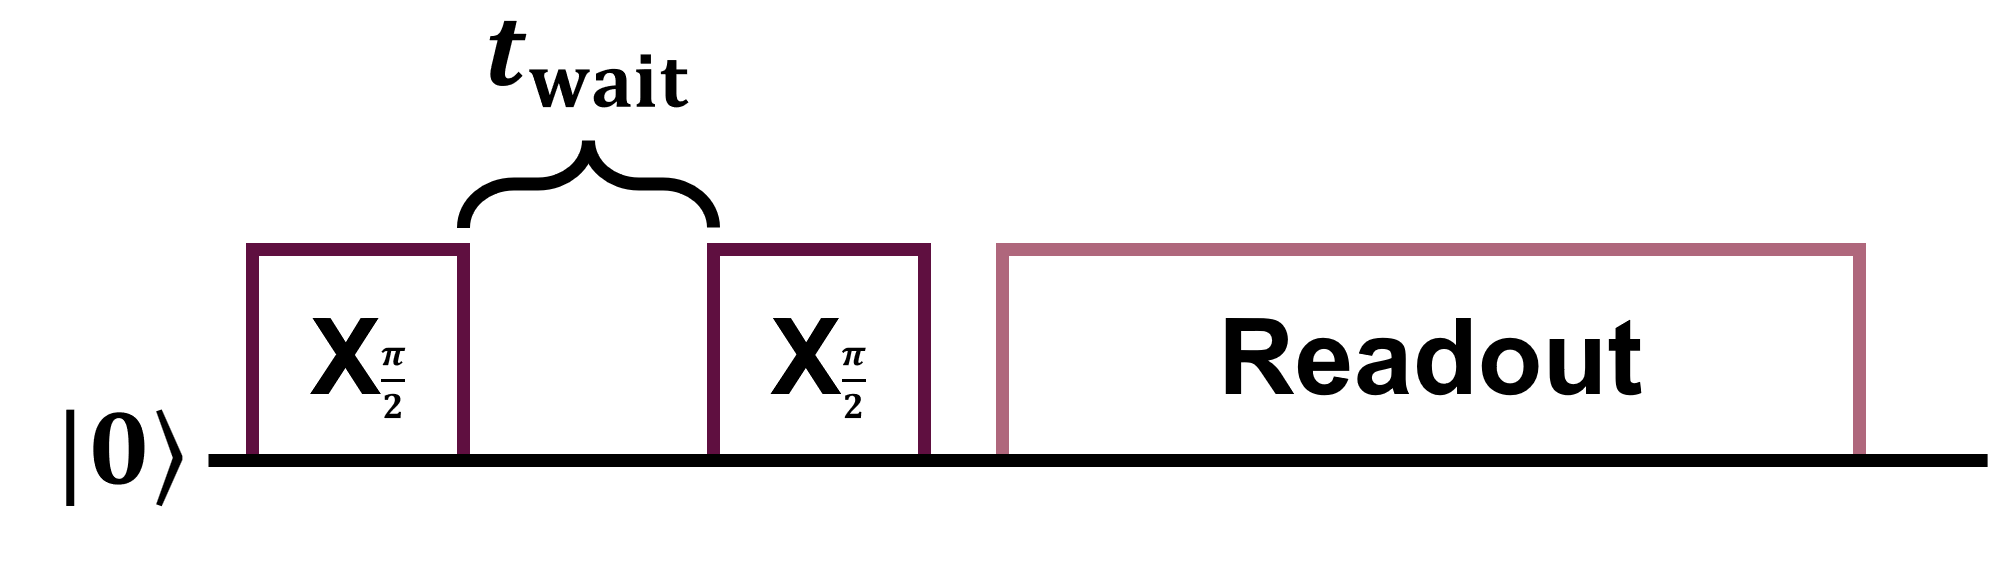
\includegraphics{Figs/circuits/t2.png}
    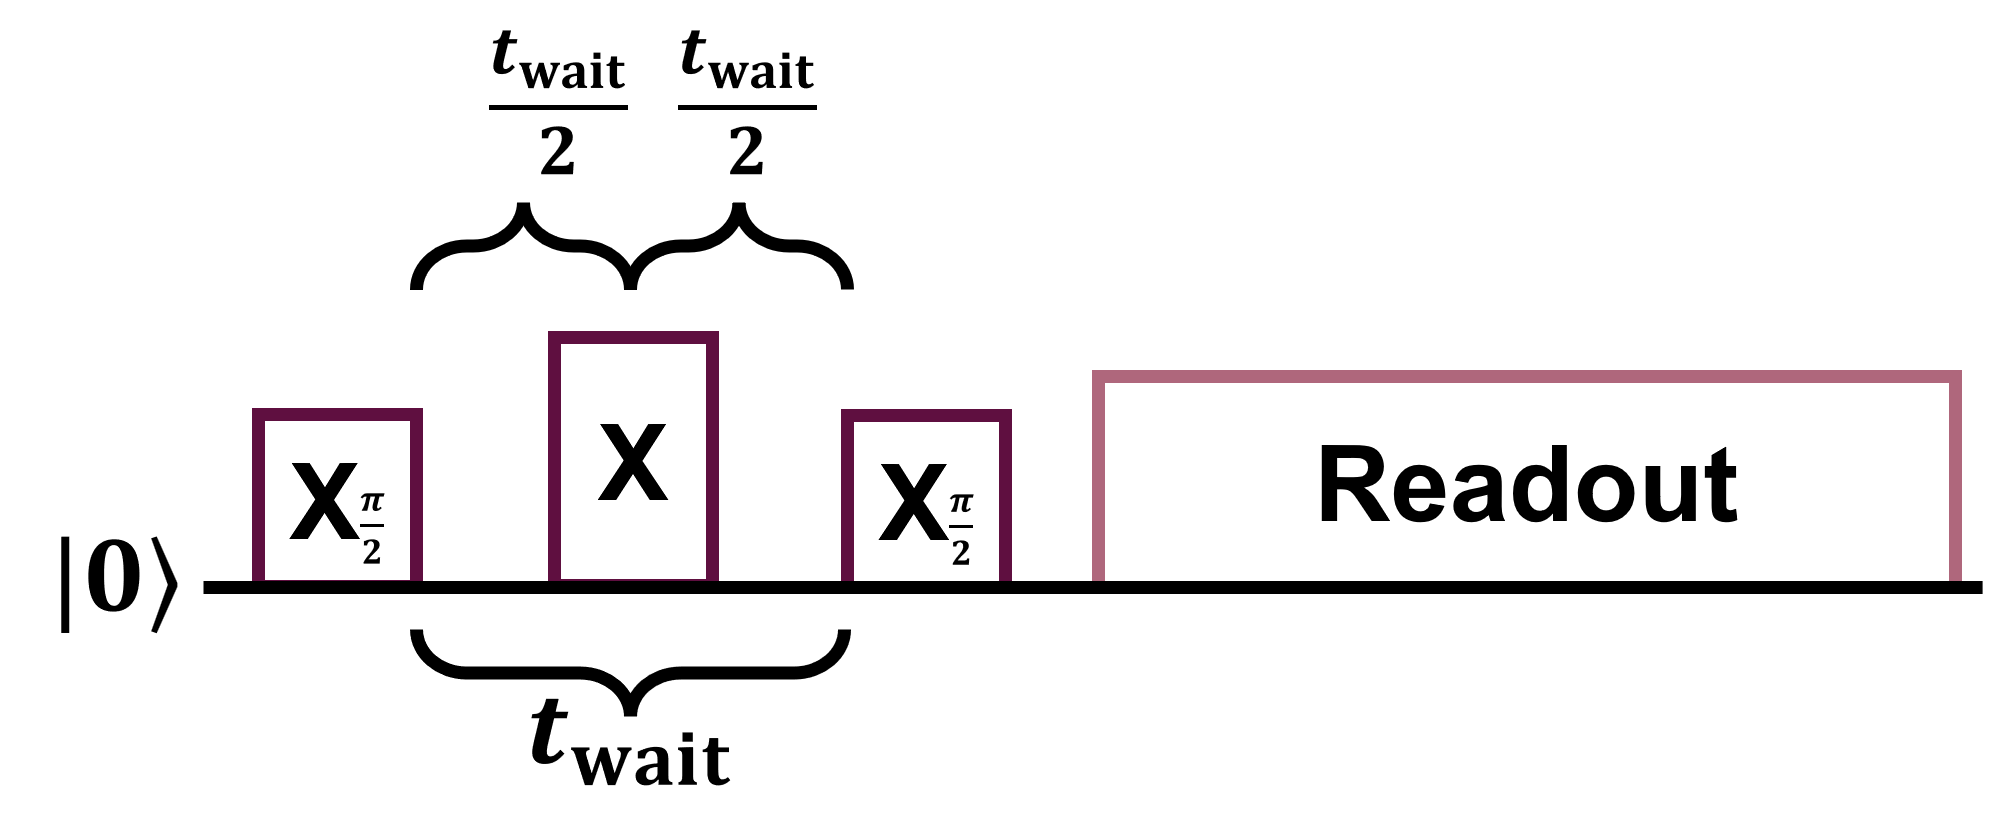
\includegraphics{Figs/circuits/t2_echo.png}
    \caption{Caption}
    \label{fig:enter-label}
\end{marginfigure}

When describing the dephasing in section \ref{sec:theory_t2} we considered two contributions: a fast changing qubit frequency shift and a slow constant shift. Thus, there also exist two methods to (and also definitions of the $T_2$. \todo{Look into the Ramsey style experiment and describe it here.}


\begin{figure*}[t]
    \begin{minipage}{0.33\linewidth}
        \centering
        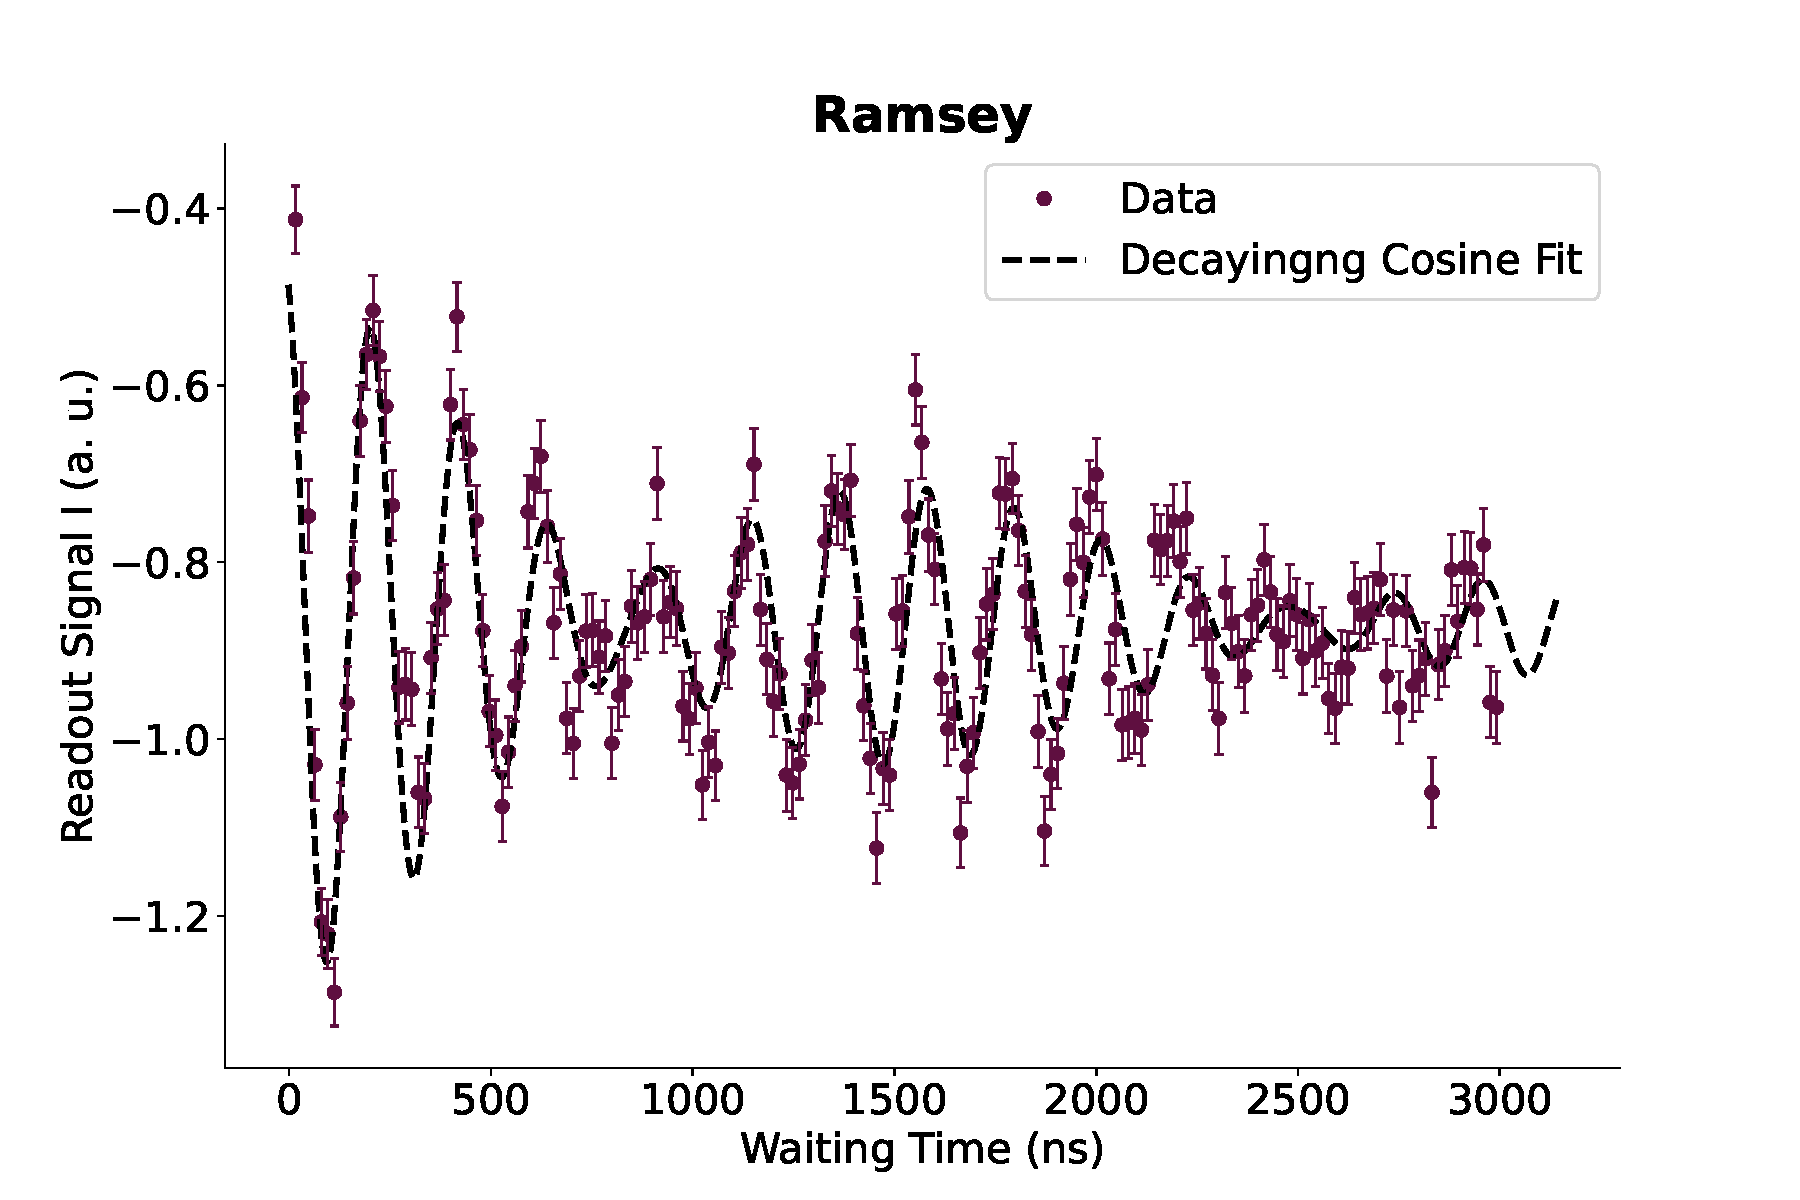
\includegraphics[width=1.0\linewidth]{Calibrations/Figures/Ramsey.pdf} % first figure itself
    \end{minipage}
    \begin{minipage}{0.33\linewidth}
        \centering
        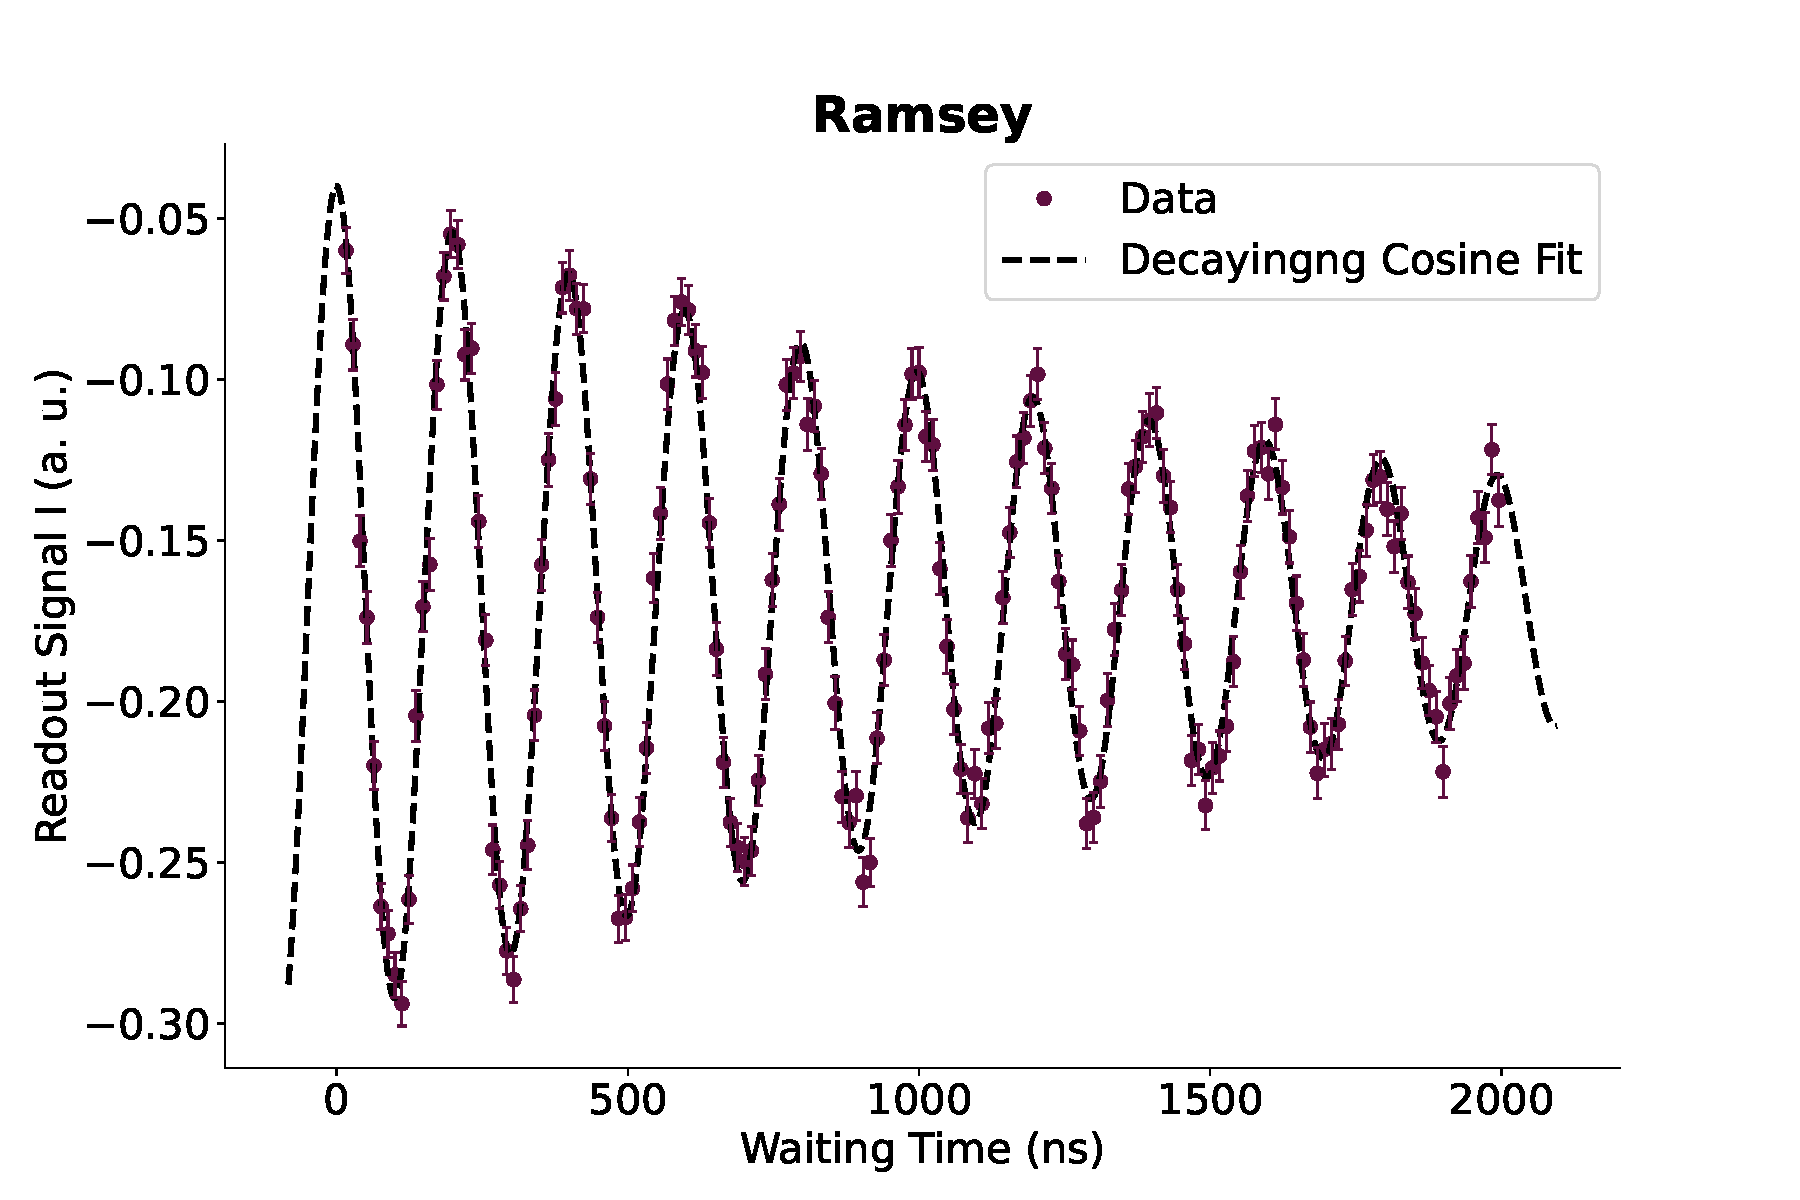
\includegraphics[width = 1.0 \linewidth]{Calibrations/Figures/old_figs/Ramsey.pdf}        
    \end{minipage}
    \begin{minipage}{0.33\linewidth}
        \centering
        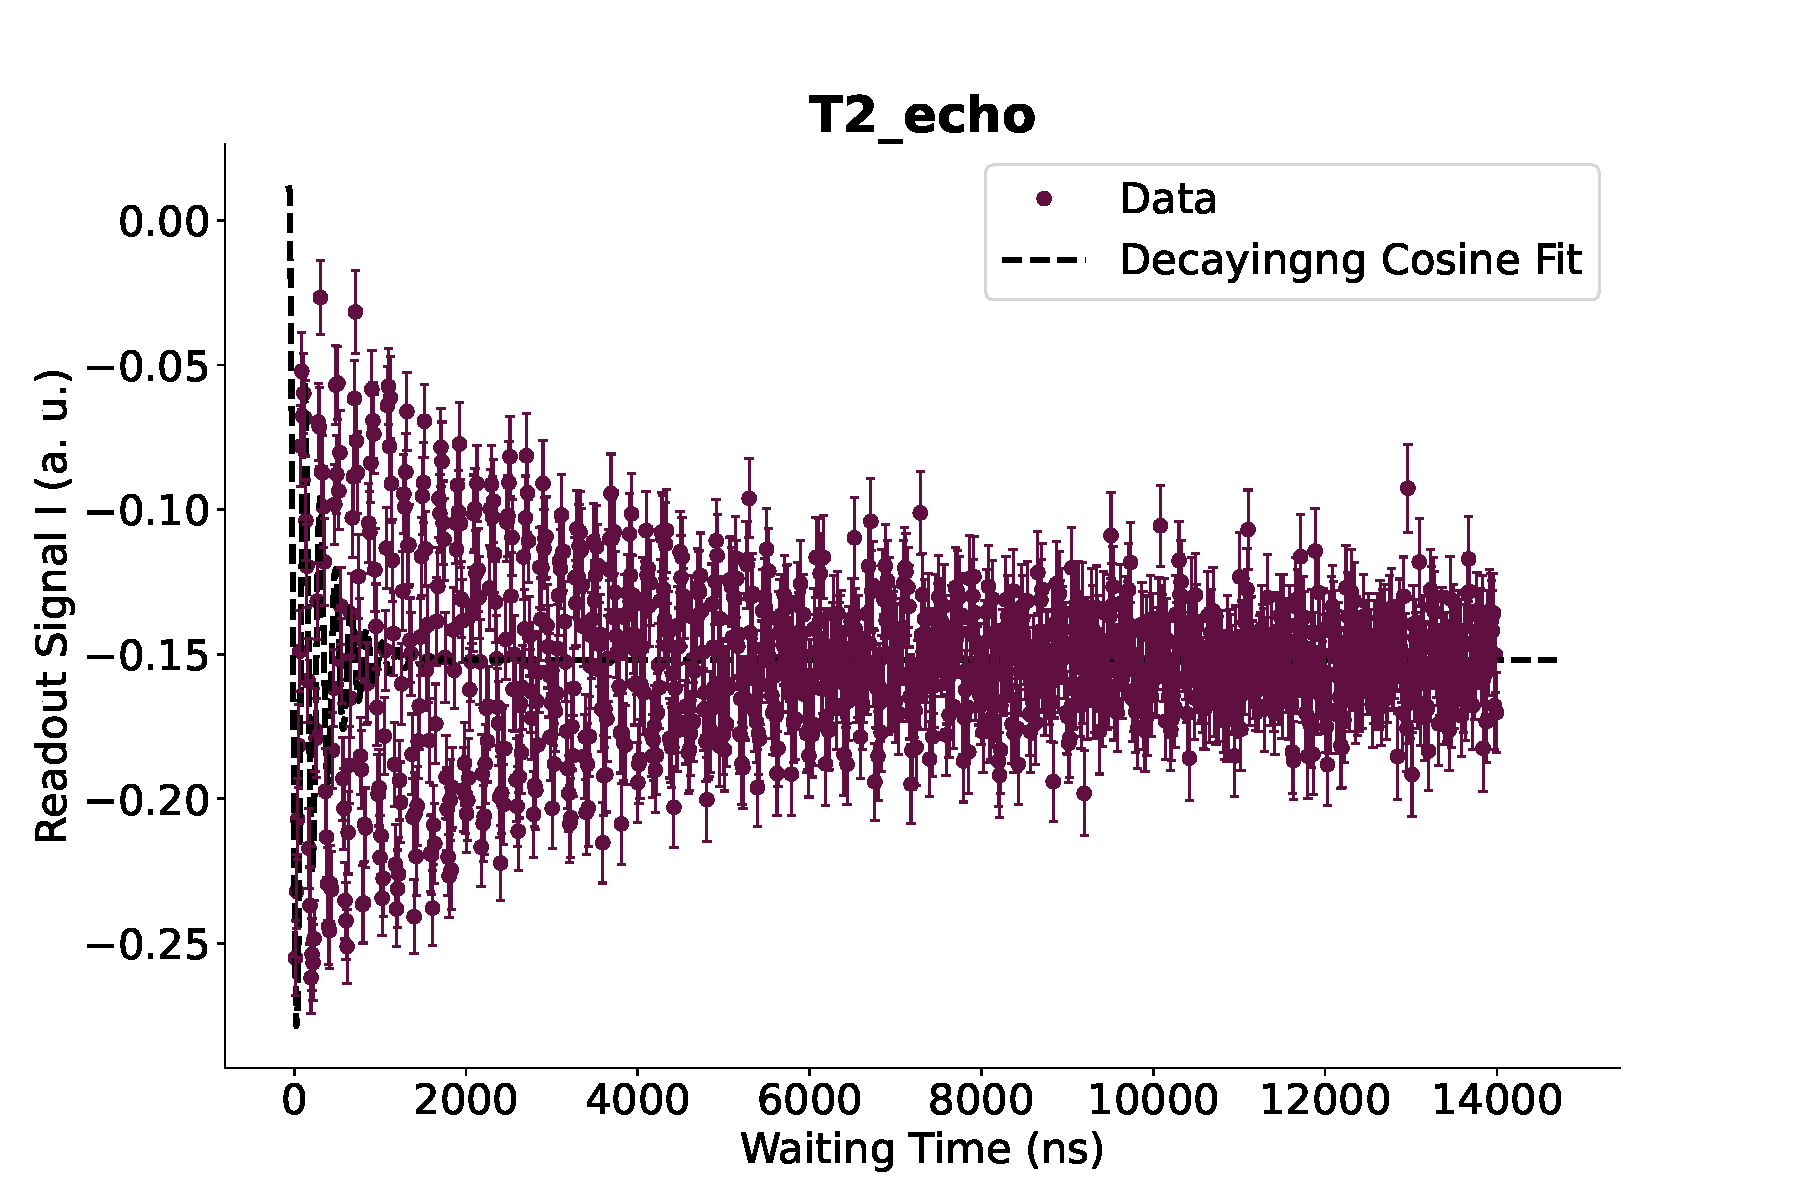
\includegraphics[width=1.0\linewidth]{Calibrations/Figures/T2_echo.pdf} % second figure itself
    \end{minipage}
    
    \caption{Figures showing the T2 experiment. The left shows the Ramsey $T_2$ while the right one shows an echo style experiment. Both are fitted with a function of the type $y = A \cos(2 \pi t f + \phi) e^{-t / T_2} + b$ where $t$ is the waiting time, $y$ is the outcome and $f, \phi, A, b$ and $T_2$ are fitting parameters.}
    \label{fig:calibrations_t2}
\end{figure*}

\paragraph{Ramsey Experiment}
This is a representative time of the qubit.
The $T_2$ time is determined by the exponential envelope in figure \ref{fig:calibrations_t2}. This is determined to be:
\begin{equation}
    T_2 = (1.65 \pm 0.12) \text{ µs} 
\end{equation}

This can further give us the dephasing time, by using equation \todo{reference $T_2$ components}
\begin{equation}
    T_\phi = \left(\frac{1}{T_2} - \frac{1}{2T_1} \right)^{-1} = (1.38 \pm 0.08) \text{ µs}
\end{equation}

\paragraph{Echo Experiememt*}
This is the limit if we allow activly chanigning the qubit to echo out the phases. We can thus eliminate low frequency noise.

\begin{equation}
    T_2^* = (2.85 \pm 0.09) \text{ µs} 
\end{equation}
\todo{Need somw good discussion here. This $T_2$ is just important when we do the efficiency calibration it is not important in simulation.}


\section{Resonator Calibration}
Next up, we characterize the resonator.

\subsection{Spectroscopy}
 Like the qubit, the frequency is the most important parameter for the resonator to determine. From the dispersive model, we however see a difference between the resonator frequency depending on which state the qubit occupies. Thus the experiment is done by doing by initializing the qubit in either $\ket{0}$ or $\ket{1}$ and performing a drive of the resonator. This leads to a dip of absorption at the resonator frequency here. Determining the resonator frequency $f_{r0}$ and $f_{r1}$, we can extract the resonator frequency $f_r$ and the dispersive shift $\chi$. This can further be used together with the resonator-qubit detuning to calculate the coupling between qubit and resonator in the dispersive approximation. This is done from $\chi = g^2 / (\omega_r - \omega_q)$.\todo{To Hz $\omega \to f$}

 The spectroscopy for the two initial states can be seen in figure \ref{fig:spectroscopy_resonator} along with a fit of lorentzian absorption. For the state $\ket{1}$, we include a secondary peak, to take the decay into $\ket{0}$ into account.
 \begin{equation}
     f_{r0} = 7.55590 \text{ GHz} \pm 3 \text{ KHz} ;\quad f_{r1} =  7.55439 \text{ GHz} \pm 11 \text{ KHz}
 \end{equation}
 \todo{These errors are way to small, we have $p$-value of 0. Redo this maybe allow the oscillating background.}
Where we can extract:
\begin{align}
    f_r  = (f_{r0} + f_{r1}) / 2 &= 7.555130 \text{ GHz} \pm 4 \text{ KHz} \\
    \chi = (f_{r0} - f_{r1}) / 2 &= (763.5 \pm 4) \text{ Khz}  \label{eq:dispersive_shift}\\
    g    = \sqrt{\chi (f_r - f_q)\left(1 + \frac{f_r - f_q}{\alpha}\right)} &= (87.0 \pm 0.4) \text{ MHz}
\end{align}

\begin{figure}
    \centering
    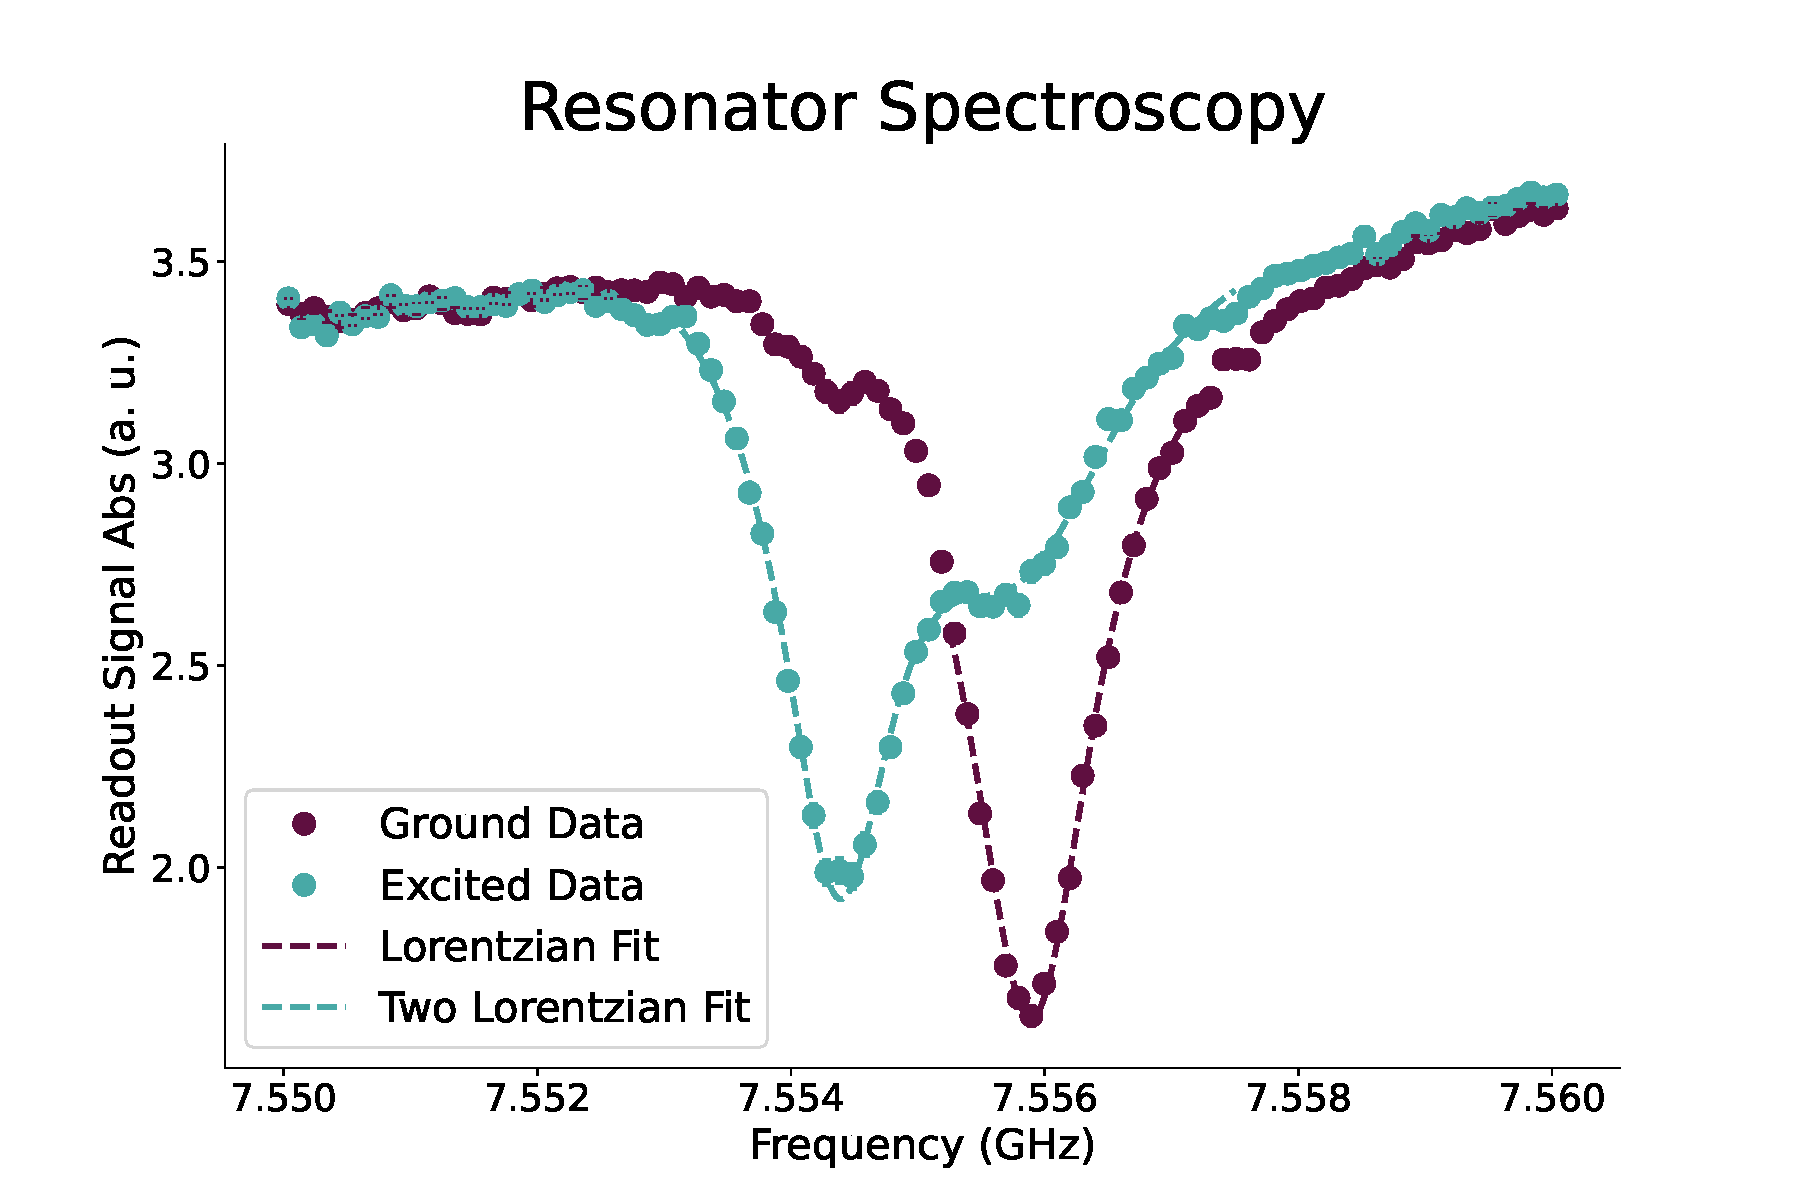
\includegraphics{Calibrations/Figures/Resonator Spectroscopy.pdf}
    \caption{Spectroscopy of the resonator signal where the qubit is either in $\ket{0}$ (purple) or in $\ket{1}$ (light blue). Since $1$ is somewhat decayed into $0$, the curve for $1$ is fitted with a douyble lorentzian. }
    \label{fig:spectroscopy_resonator}
\end{figure}
\todo{The label is wrong here, it should be absolute value.}

\subsection{Resonator Decay Rate}
\begin{figure}
    \centering
    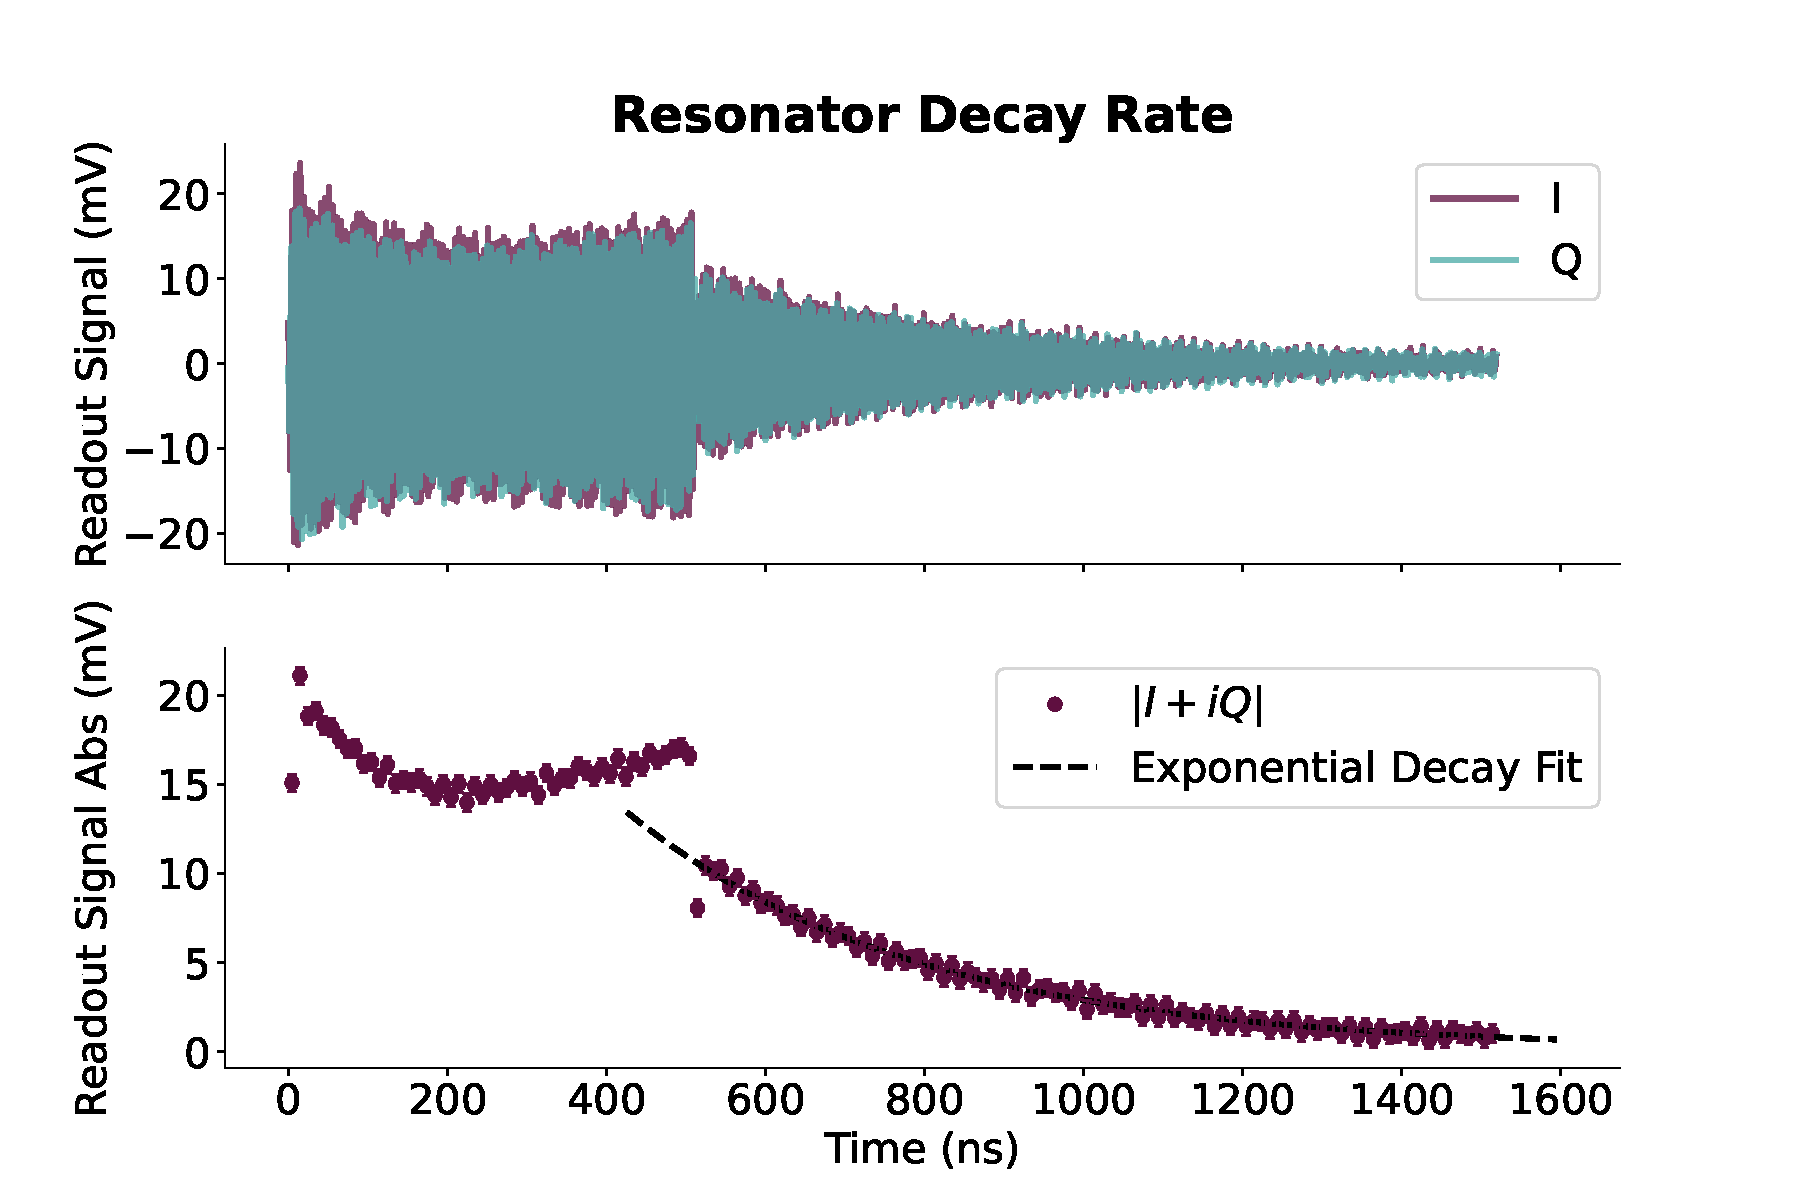
\includegraphics{Calibrations/Figures/Resonator Decay Rate.pdf}
    \caption{Traces from a short drive and a following monitoring of the feed line. In the top panel, the meaned $IQ$ traces are taken. In the lower, the $|I(t) + iQ(t)|$ values are plotted and averaged over $10 \text{ ns}$ intervals. The last part (from $t = 600 \text{ ns}$ is fitted with an exponential function: $y = Ae^{-\kappa t} + b$ where $t$ is the time $y$ is proportional to the mean photon number and $A, b$ and $\kappa$ are fitting parameters.}
    \label{fig:calibration_of_kappa}
\end{figure}
We now turn our eyes to the resonator depletion rate, $\kappa$. We found in section \ref{}\todo{reference} that the resonator will decay exponentially when not driven. Thus we extract this parameter by applying a constant pulse to the resonator. After it is excited, we stop the pulse but continue to monitor the $I$ and $Q$ signal. Remembering that the average photon number can be found from the distance to origo in the $I-Q$-plane, we plot $\Bar{n}(t) = |I(t)+iQ(t)|$. An average of 10,000 trace from this experiment is displayed in \ref{fig:calibration_of_kappa}. The traces are coarse grained over a $10 \text{ ns}$ interval to cancel some unwanted oscillating behaviour. Fitting the last part of the data, we obtain:
\begin{equation}
    \kappa = 3.8 \pm 0.6 \text{ MHz}
\end{equation}


We can also compare this to the width of the resonator dips. With the Lorentzian distribution the width is given as $2 \pi \kappa$. Comparing in the fit, we would get $\kappa = (3,87 \pm 0.08) MHz$ from the dip of $\ket{0}$ and $\kappa = (3.50 \pm 0.07) MHz$ from $\ket{1}$ which is not as reliable since the two distributions used to fit probably mixes.   

\subsection{Photon Counting}
With the above calibrations, it is possible to recreate much of the dynamics in the qubit and in the resonator in simulation. This is at least qualitatively. When taking the expectation value of a density matrix, we would give some value of the system like $\expval{\sigma_z}$ or $\expval{I} + i\expval{Q}$. In experiment, we often use the I and Q values given in units voltage. Now, we will try to bridge the gap for the resonator values. To do this, we will make use of two properties: 
\begin{enumerate}
    \item In section \ref{}\todo{Write and refer to this}, we described how the resonator goes into a steady state when driven. In the IQ plot, the mean photon number was proportional to the driving amplitude. 
    \item Like the qubit state shifts the resonator frequency, the qubit frequency is also shifted in we were to fill the resonator with photons. We can thus, rewrite equation \ref{eq:two_level_qubit_dispersive} to the convenient form: $H = \Tilde{\omega}_r a^\dagger a  + \left(\frac12 \Tilde{\omega}_{01} + \chi a^\dagger a\right)  \sigma_z$
\end{enumerate}
These two properties can be combined by driving the resonator into its steady state. When the steady state is reached, we can do a a spectroscopy experiment on the qubit (like described in section \ref{sec:calibration_qubit_spectroscopy}). But since the resonator is filled, the qubit frequency will be shifted and by measuring the qubit afterwards, we find a peak at the "new" qubit frequency. Repeating this experiment for different resonator drive amplitudes, we can extract a relation between amplitude and mean photon number in the steady state. The two-dimensional scan of the readout signal can be seen in figure \ref{fig:calibration_photon_counting_scan}.

\begin{marginfigure}[-4 cm]
    \centering
    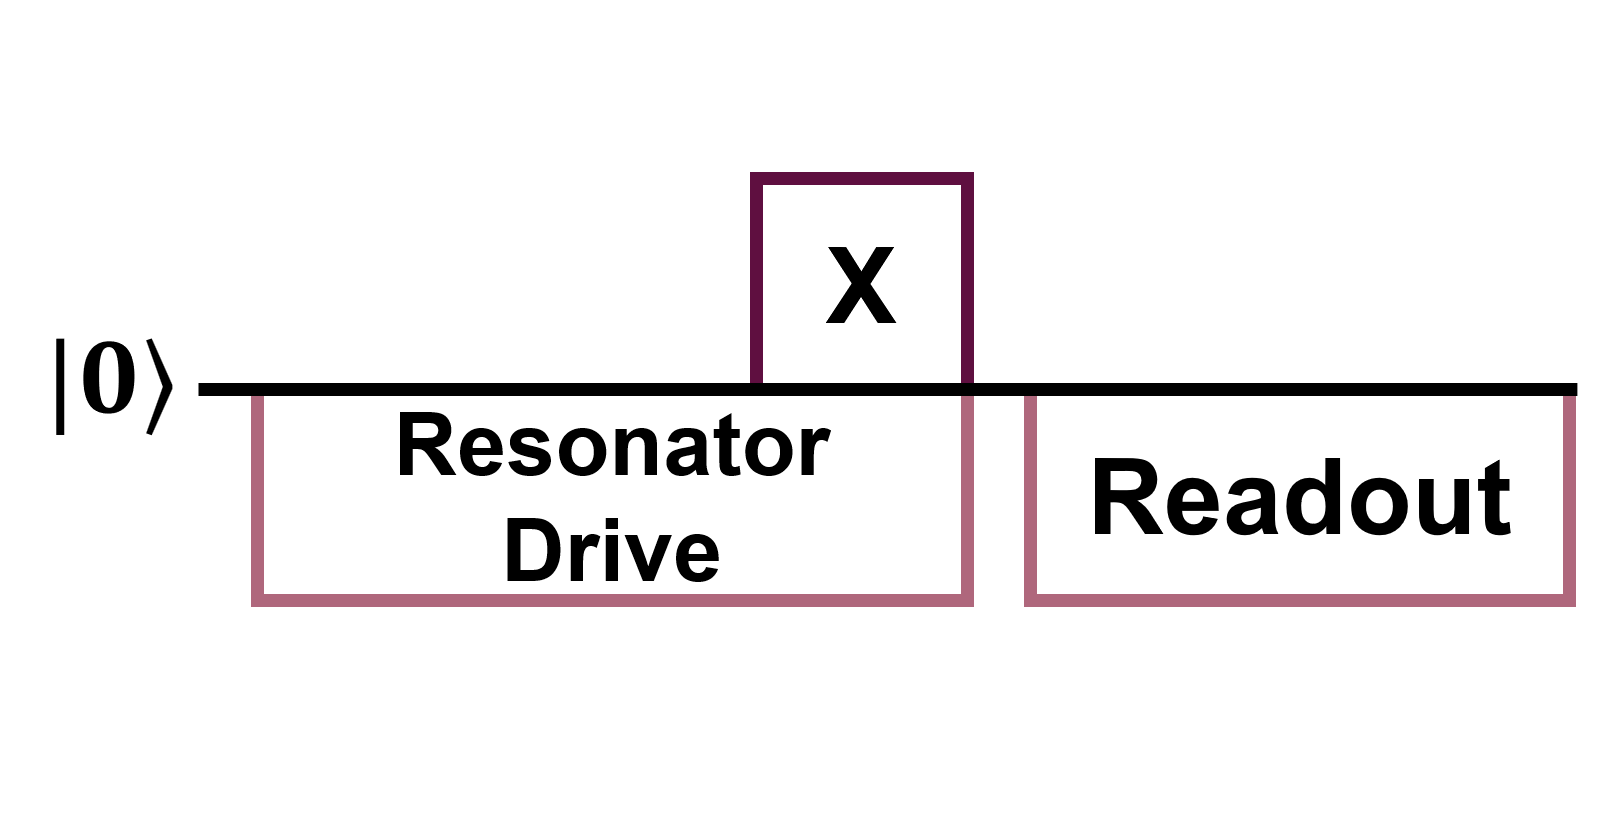
\includegraphics{Figs/circuits/photon_counting.png}
    \caption{Caption}
    \label{fig:enter-label}
\end{marginfigure}

\begin{figure}[h]
    \centering
    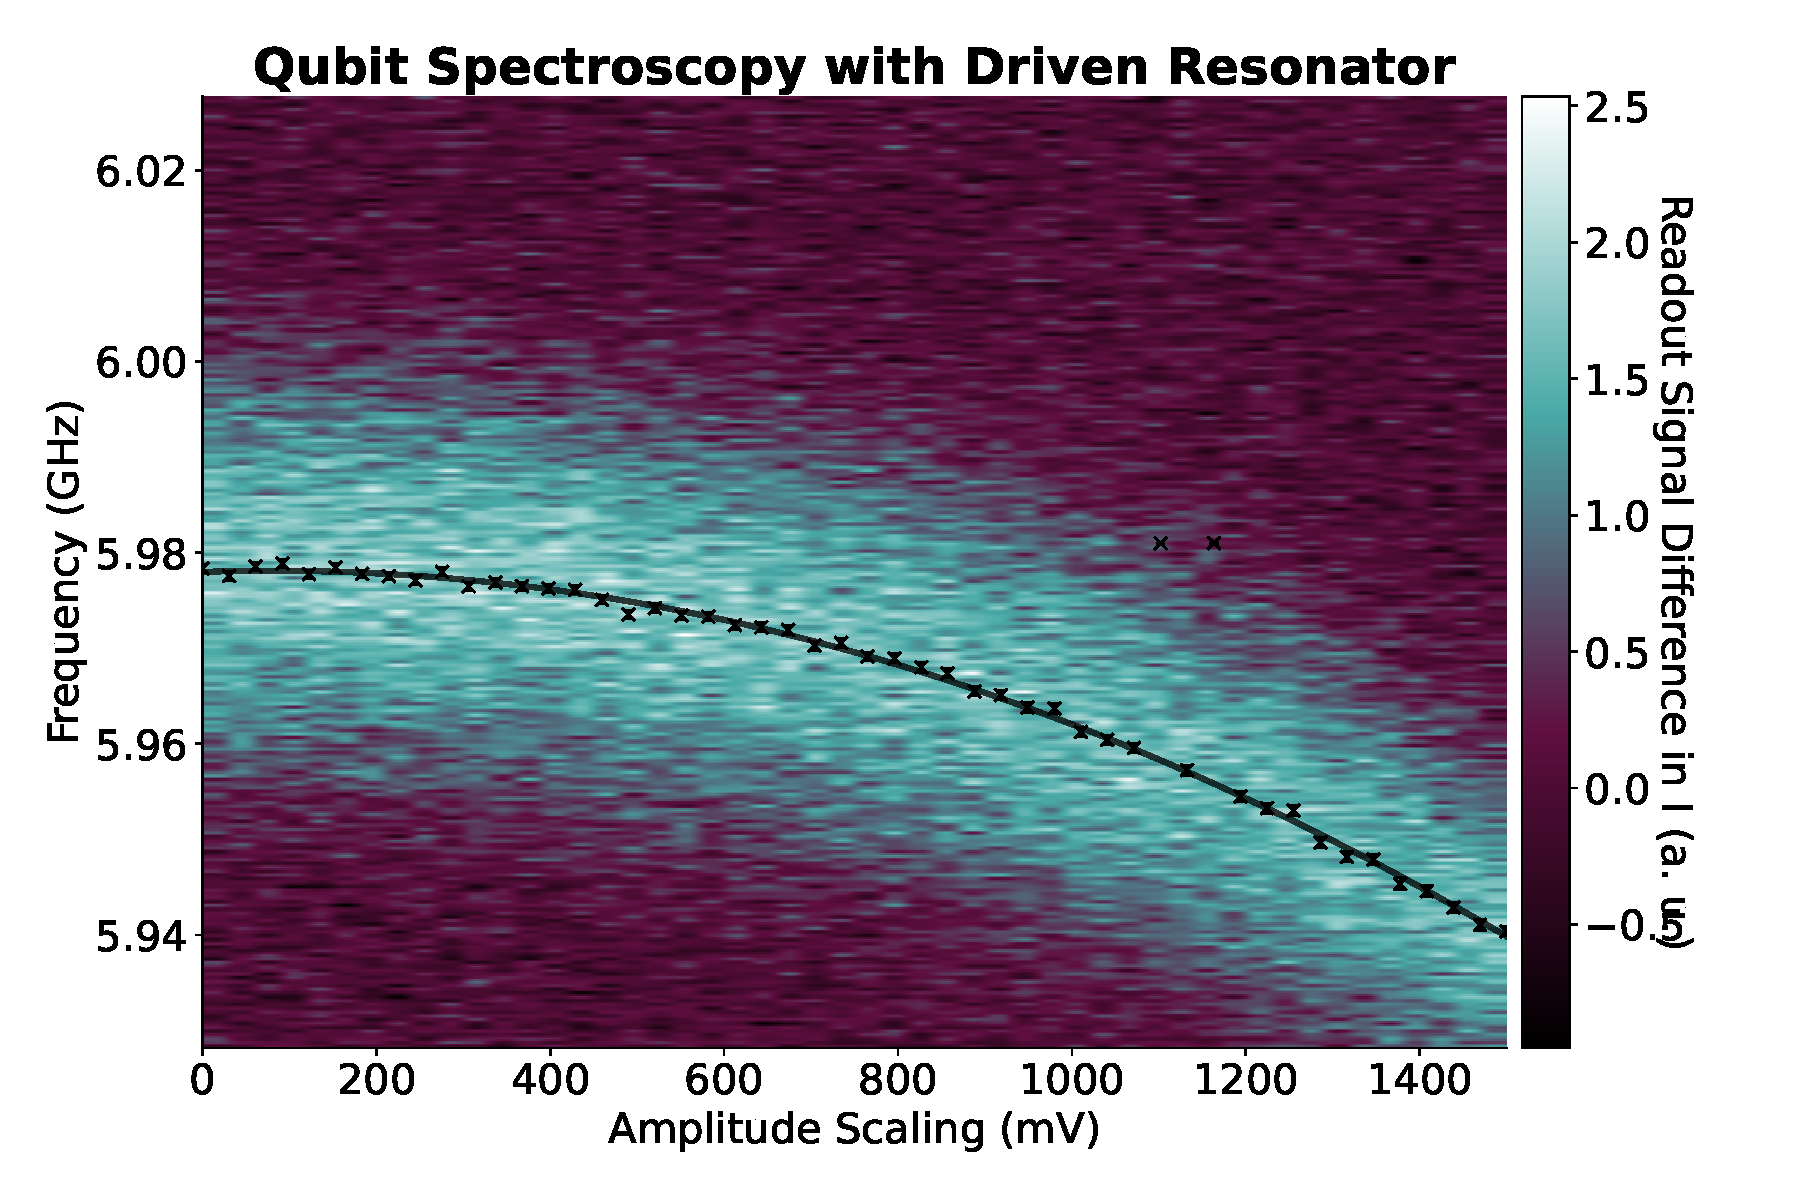
\includegraphics[]{Calibrations/Figures/Qubit Spectroscopy with Driven Resonator.pdf}
    \caption{Scan of readout-pulse-amplitude and the frequency of qubit-pulse.}
    \label{fig:calibration_photon_counting_scan}
\end{figure}

If we now fit a Lorentzian curve over the frequencies for each amplitude and divide with the dispersive shift from equation \ref{eq:dispersive_shift}, we can obtain the relation between steady state photon number and the readout amplitude. This fit can be seen in figure \ref{fig:calibration_amplitude_photon_number}. \textit{By further extracting the $|I+iQ|$ value at each amplitude in a regular readout, we can also get a linear equation. By combining the two slopes we can scale the voltage values to resonator photon count. This also allows us, to find the amplitude $\epsilon$ experienced in the drive, which is a more complex combination of physical parameters on the chip as well as the applied feed line voltage.}

\begin{figure}
    \centering
    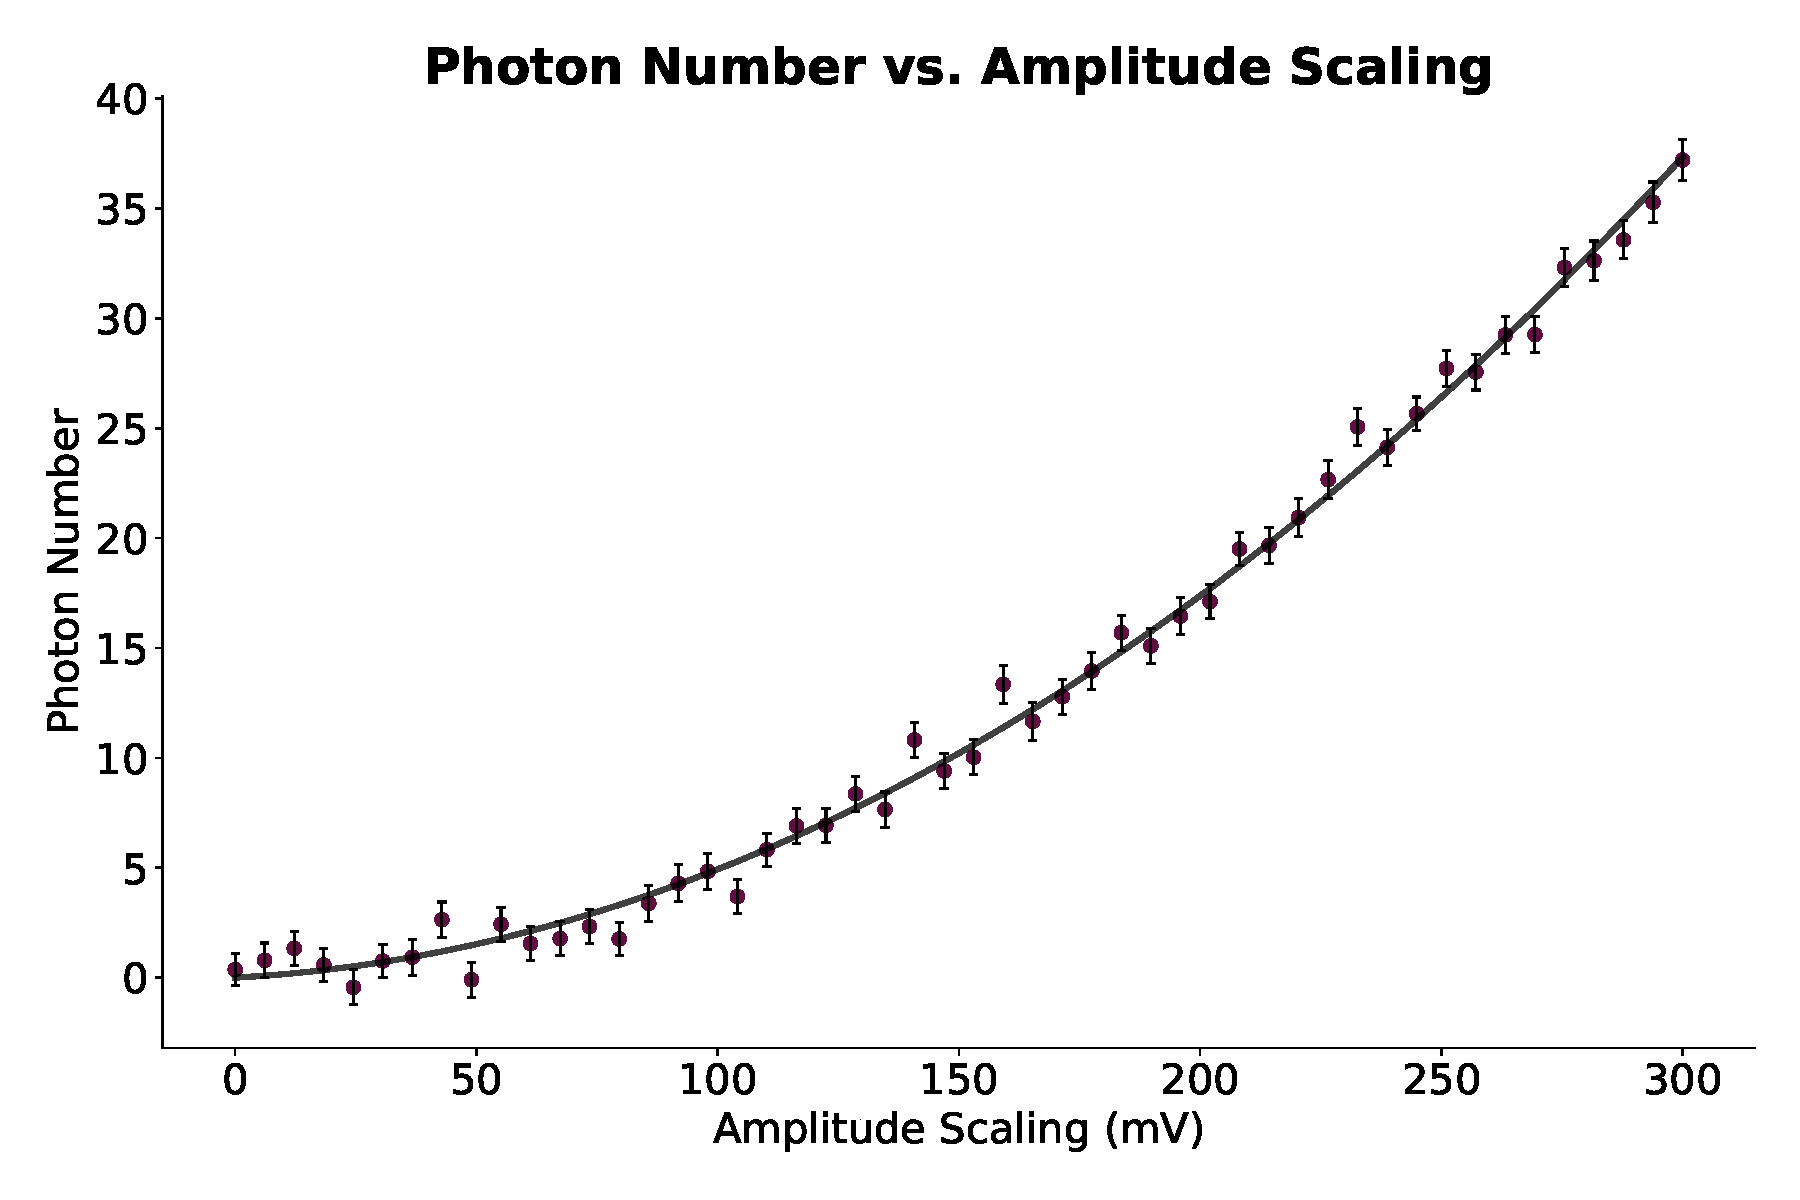
\includegraphics[]{Calibrations/Figures/photon_number.pdf}
    \caption{Caption}
    \label{fig:calibration_amplitude_photon_number}
\end{figure}

By doing the analysis, we can fit a polynomial to get the form of the curve. This allows us to estimate the value at $100\%$ of the actual readout amplitude. This allows us to estimate the mean photon number of the readout end of the readout to be:

\begin{equation}
    \Bar{n} = 21 \pm 1
\end{equation}

While we are not in a perfect steady state this still allow us to find the drive experiences by the resonator:

\begin{equation}
    \epsilon = \Bar{n} \sqrt{\left(\frac{\kappa}{2}\right)^2 + (\chi)^2} = 6.4 \text{ MHz}
\end{equation}
When driving the resonator at its frequency $f_r$.


% One big challenge still stands, how do we map the axis to each other?  


% Considering the dispersive hamiltonian of the qubit-resonator-system, Eq. \ref{eq:two_level_qubit_dispersive}, we have above primarily considered the shift of resonator frequency depending on the qubit state, but just moving the parenthesis to represent it in the form:
% \begin{equation}
%     H = \Tilde{\omega}_r a^\dagger a  + \left(\frac12 \Tilde{\omega}_{01} + \chi a^\dagger a\right)  \sigma_z
% \end{equation}
% making it apparent that while the qubit state moves the resonator, the opposite is also true. Since the qubit frequency moves with $\chi$ for each photon in the resonator, we 




% The protocol is carried out in the following way:
% \begin{itemize}
%     \item Drive the resonator at a given amplitude to fill it with photons.
%     \item When the resonator is in its steady state apply an X-gate with a given frequency.
%     \item Perform a regular readout
% \end{itemize}
% By sweeping over amplitude and X-gate frequency, one can find the resonance frequency at every amplitude. Since the resonance frequency is related to the qubit \\

% % \begin{marginfigure}[- 5 cm]
% %     \centering
% %     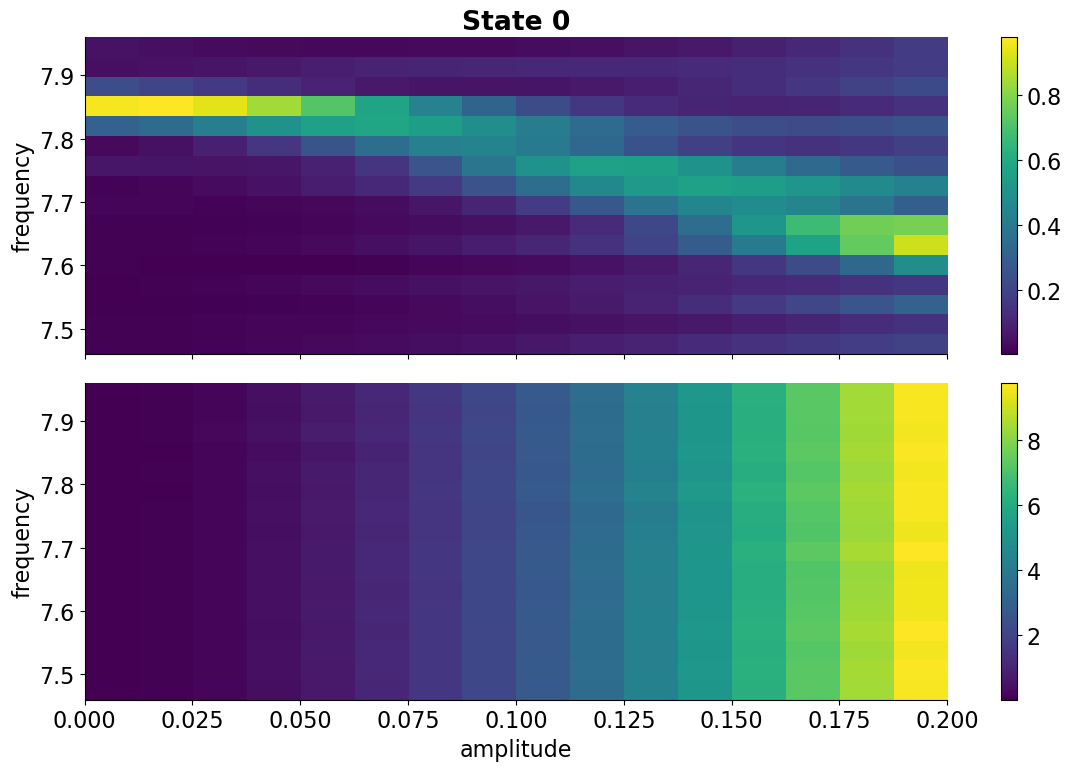
\includegraphics[width = 1.3 \textwidth]{tex/fig_for_text/section_6/photon_number_calibration.png}
% %     \caption{Simulation of photon number calibration protocol.  }
% %     \label{fig:photon_number_calibration}
% % \end{marginfigure}

% \noindent
% \textbf{We need the following Data}:
% \begin{itemize}
%     \item First calibrate the double dip and find the dispersive shift from above
%     \item For the $\ket{0}$, we should drive the resonator at the resonator frequency and measure the $|I + iQ|$
%     \item For the $\ket{1}$, we fill the resonator with photons and apply an x-gate with a given frequency. Scan over this frequency to find the resonance frequency as a function of amplitude $\to |I + iQ|$ measured above
%     \item We should repeat this experiment where we apply another readout frequency to the most optimal (probably in between the two peaks). 
% \end{itemize}

\section{Readout Efficiency}
The amplification chain from the qubit and resonator up to our digitization of the signal is by no means lossless. As mentioned in section \ref{sec: Amplifiers}\todo{Write section about amplifiers} there is a lower bound on the amount of noise added by an amplification. But in addition, the signal sees multiple amplification and thermalization at different stages ultimately giving us a much noisier signal than what is actually extracted from the qubit. To include this effect in our simulation and just to benchmark the amplification chain we will extract the quantum efficiency, $\eta$ by a method presented in \cite{bultink},\todo{Cite properly the Bultink et al. article} where the backaction of the qubit is compared to the Signal to Noise Ratio of the output signal. 

\begin{marginfigure}
    \centering
    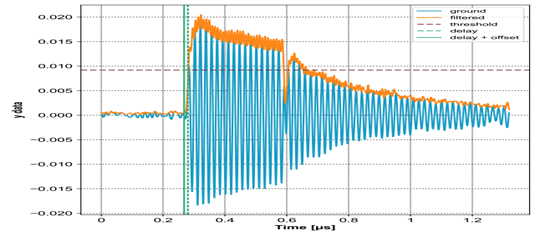
\includegraphics{Figs/calibrations/efficiency/pulse_shape.png}
    \caption{The signal in the resonator during the readout signal.}
    \label{fig:efficiency_pulse_shape}
\end{marginfigure}

To use this method, one must first create a readout pulse with a signal that is zero at start and end: $S(t = 0) = S(t = T) = 0$. To limit decoherence during the readout, one would choose a short pulse and readout during a cooldown of the resonator for $\approx 5 / \kappa$.\todo{One can optimzie this further by applying a stimulated depopulation pulse. Write this in here if we do it.} The shape and resonator signal in pulse is shown in figure \ref{fig:efficiency_pulse_shape}. \todo{Add pulse shape as well}

Given the readout signal, the extraction now consist of two parts:
\begin{enumerate}
    \item Determine how the SNR changes when we increase the readout amplitude. With a signal starting and ending at 0, this should follow a linear relation: $\text{SNR}(\epsilon) = a \epsilon$.
    \item Investigate the backaction of the readout on the qubit. After a pulse, the coherence is related to the readout amplitude by the gaussian relation $|\rho_{01}(T, \epsilon)| = |\rho_{01}(T, 0)|e^{-\epsilon^2/2\sigma^2}$
\end{enumerate}

Which is related to the quantum efficiency by\cite{boltink}\todo{Derive either here, in appendix or above in the theory section}:
\begin{equation}
    \eta = \frac{a^2\sigma^2}{2}
\end{equation}

\subsection{Amplitude Dependence of SNR}
To determine the SNR from the readoutpulse, one does a simple experiment, which is close to what we have done before. \todo{Refer and make a connection} By initializing the qubit in $\ket{0}$ and then performing an $X$-gate to every other initialization before reading it out, one can see determine the separation between $\ket{0}$ and $\ket{1}$ (see figure \ref{fig:efficiency_SNR_experiment})

\begin{marginfigure}
    \centering
    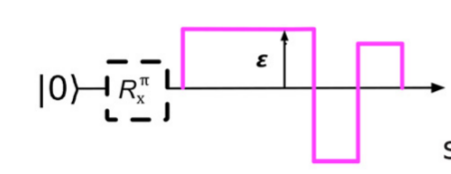
\includegraphics{Figs/calibrations/efficiency/experiment_circuit_SNR.png}
    \caption{Circuit for experiment}
    \label{fig:efficiency_SNR_experiment}
\end{marginfigure}

Repeating the experiment $n$-times for different values of $\epsilon$, we obtain the results in figure \ref{fig:effiiency_results_SNR}, where the distribution for the last $\epsilon$ is shown together with the relation between calculated SNR and applied amplitude. Fitting a linear equation to the results, we obtain $a = ??$. \todo{Extract value from $a$ with errors and write samples, make prettier figure.} 

\begin{figure*}
    \centering
    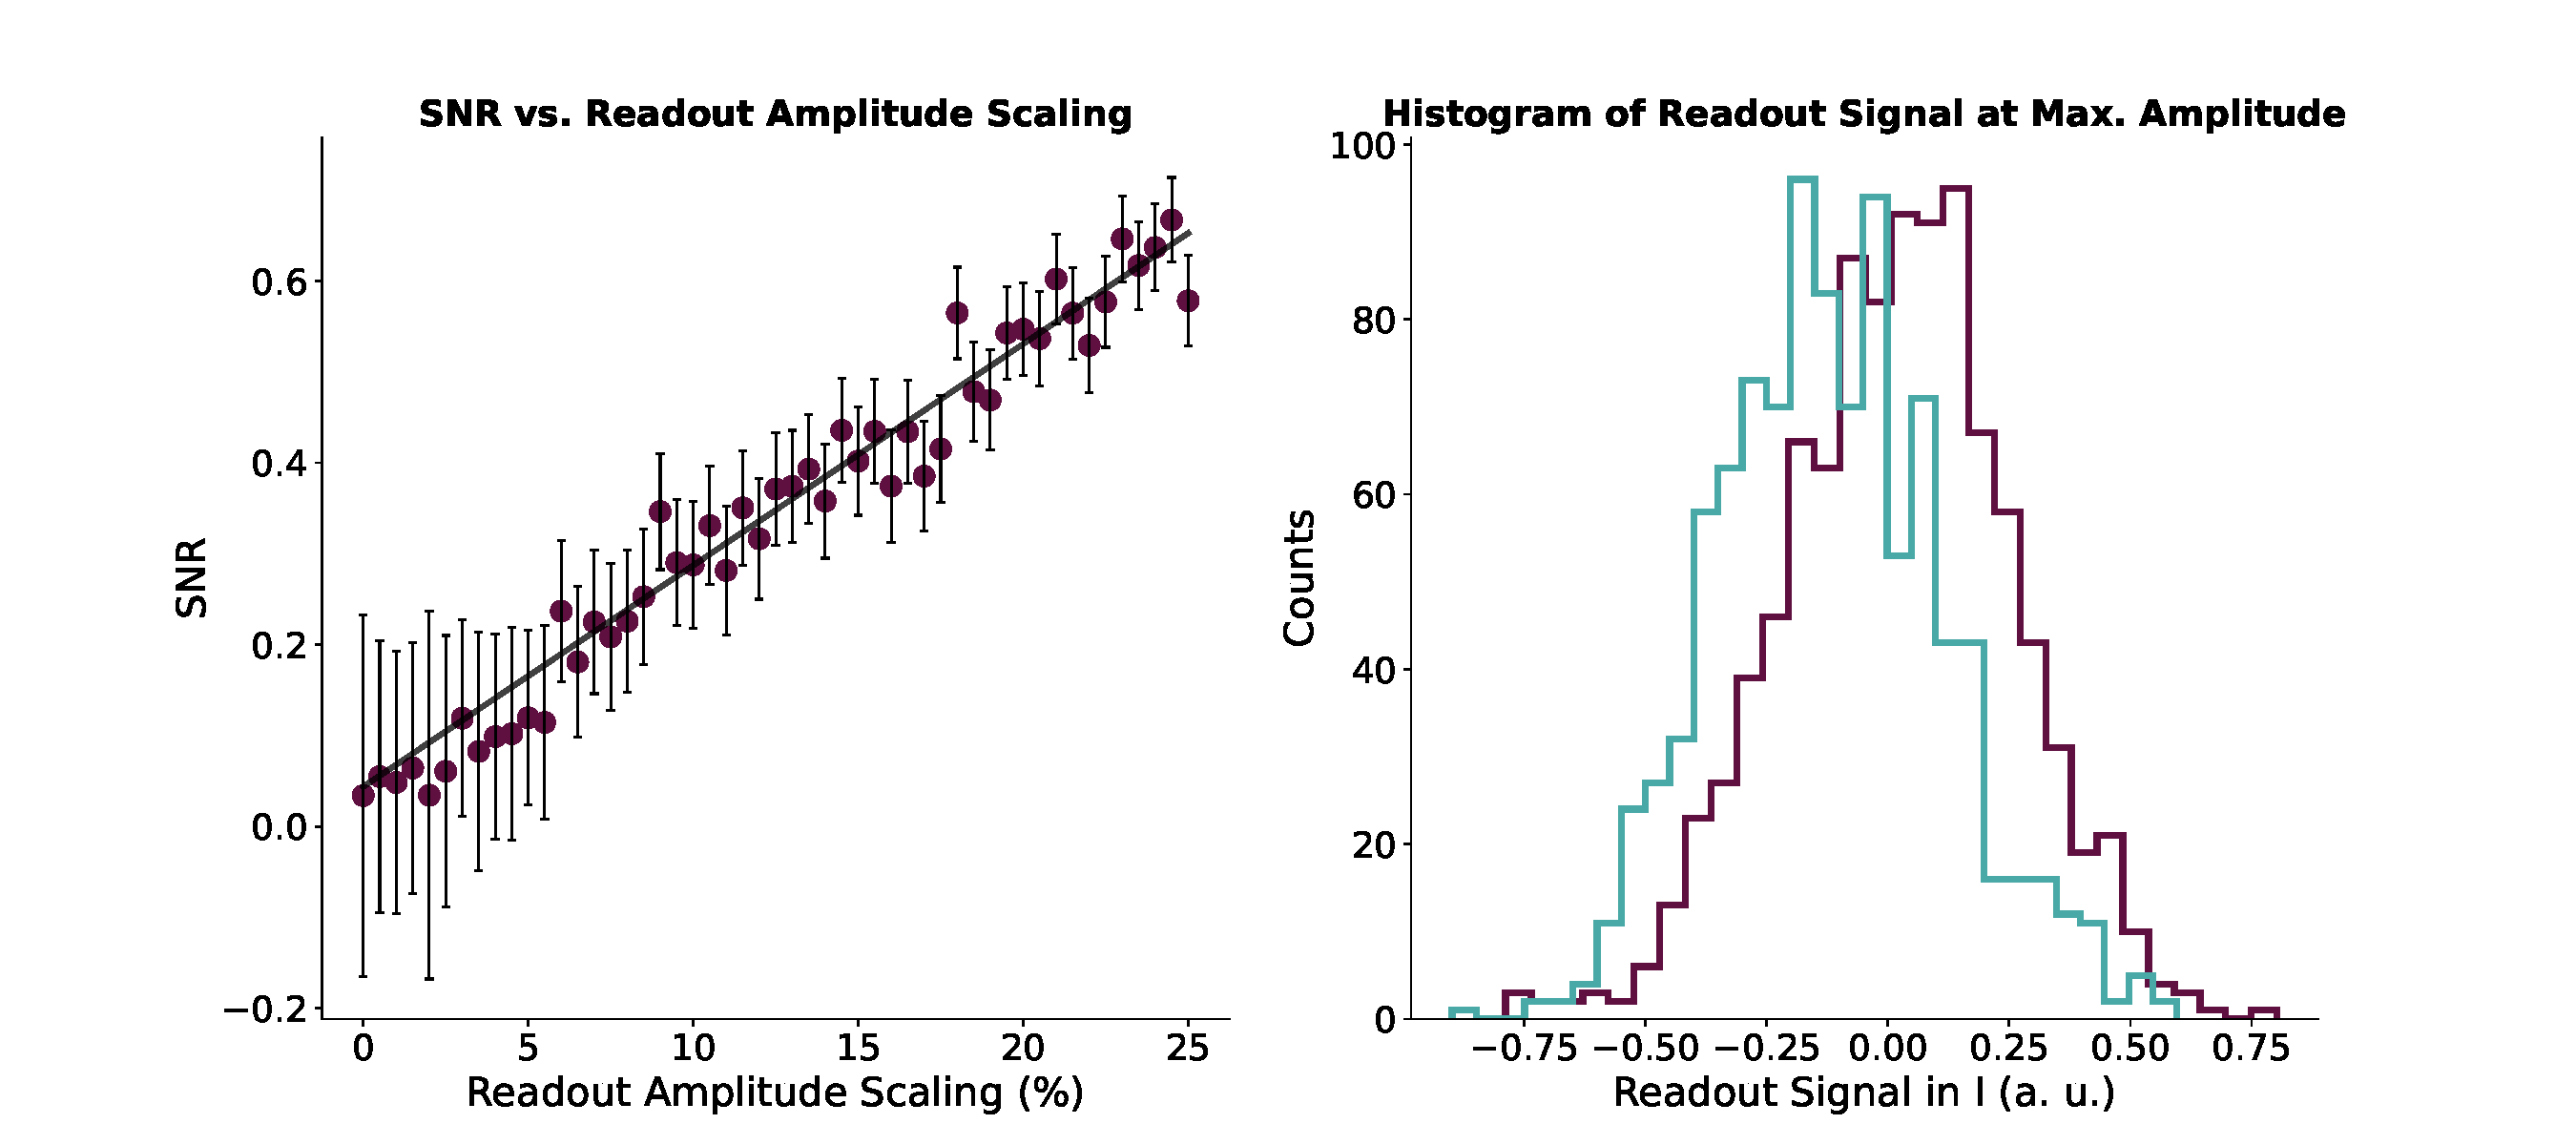
\includegraphics{Calibrations/Figures/SNR_vs_amplitude.pdf}
    \caption{Figure showing the experiment for extracting SNR as a function of readout ampltiude. An example at the highest amplitude is shown, where the two distributions are separated. The SNR is extracted as $\text{SNR}^2 = \expval{S_{\ket{0}} - S_{\ket{1}}}^2/\left(\expval{S^2_{\ket{0}}} +\expval{S^2_{\ket{1}}}\right)$. The other figure displays the result of this analysis for all values of $\epsilon$ as well as a linear fit applied to it.}
    \label{fig:effiiency_results_SNR}
\end{figure*}



\subsection{Backaction from Readout Pulse}
\todo{When writing the Backaction section together with the stochastic equation, make sure everything needed here is covered. Connect this section back.}
For finding the relation between the amplitude and backaction, the qubit is initialized in $\ket{0}$ and a $R^x_{\pi/2}$ pulse is performed to send the qubit into $\frac{1}{\sqrt{2}}\left(\ket{0} + \ket{1}\right)$. With the pulse in this state, the density matrix will be:
\begin{equation}
    \rho(t=0) = \frac12 \begin{pmatrix}1 & 1 \\ 1 & 1\end{pmatrix}
\end{equation}
the readout drive will now be applied\footnote{Just as pulse because we're not interested in the signal}. During the readout signal the off-diagonal elements will be reduced by two factors: inherent dephasing by $T_2$-processes and qubit back action by the signal. To determine the amount of dephasing, we will perform a $\pi/2$ rotation around the axis $\phi$ in the x-y-plane before reading out the signal. The entire sequence is illustrated in figure \ref{fig:efficiency_dephasing_experiment}.

\begin{marginfigure}
    \centering
    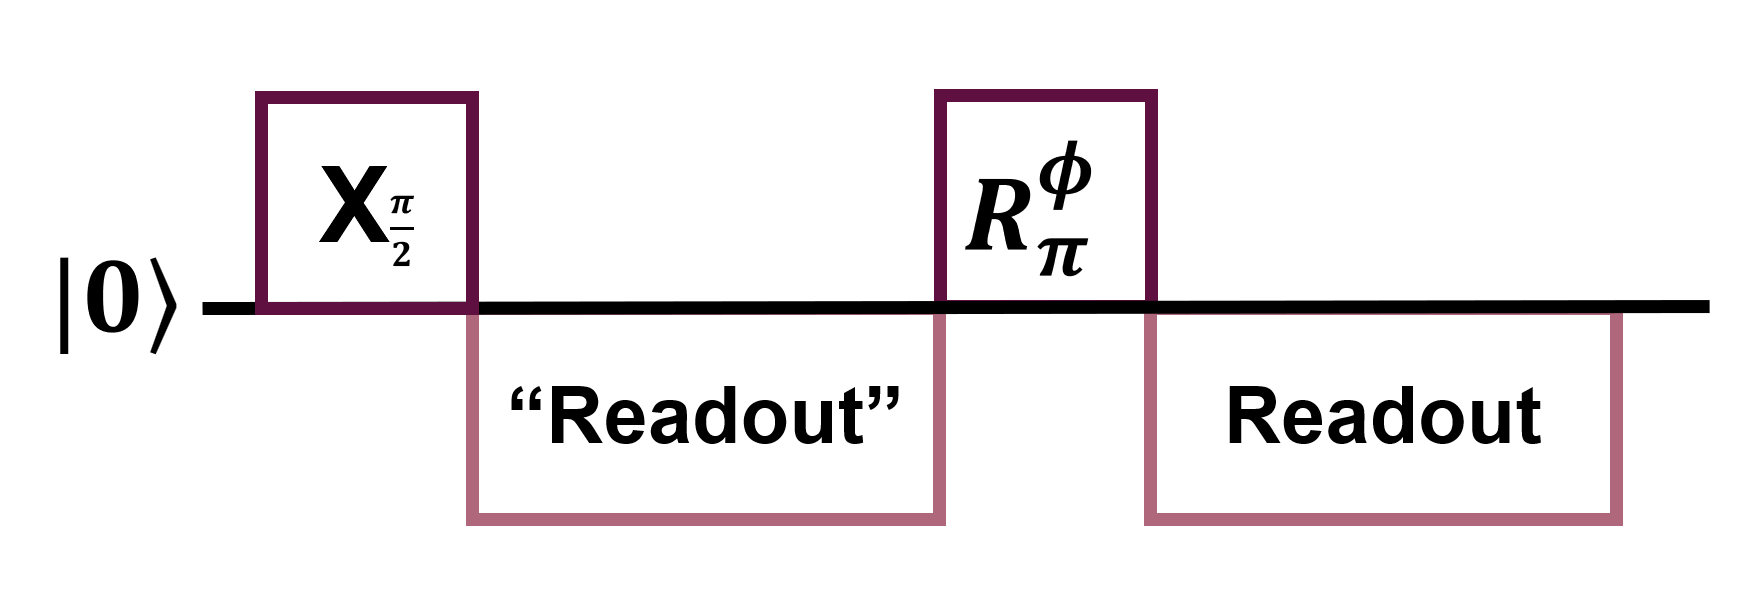
\includegraphics[]{Figs/circuits/dephasing.png}
    \caption{The phasing experiment circuit. First the qubit is rotated $\pi/2$ around the X-axis, whereafter it is subject to the readout pulse without demodulating and saving the signal. Now the qubit is rotated $\pi$ around a vector $\phi$ in the $x-y-$plane and finally readout.}
    \label{fig:efficiency_dephasing_experiment}
\end{marginfigure}

Reading out the signal for different angles of $\phi$ will lead to a cosine shape: $\sigma_z = 2 |\rho_{01}(t= T)| \cos(\phi+\phi_0)$. And repeating for different readout amplitudes the dephasing due to backaction can be separated from the one due to $T_2$-dephasing which only has an effect of the amplitude. The results of the experiment can be seen in figure \ref{fig:efficiency_dephasing_experiment}, where the parameter from the important parameter for the Gaussian fit is the standard deviation: $\sigma = 0.0045 \pm ?$. \marginnote{Write the $\chi^2$ and $p-val$ for the fit in the marginnote.}

\begin{figure*}
    \centering
    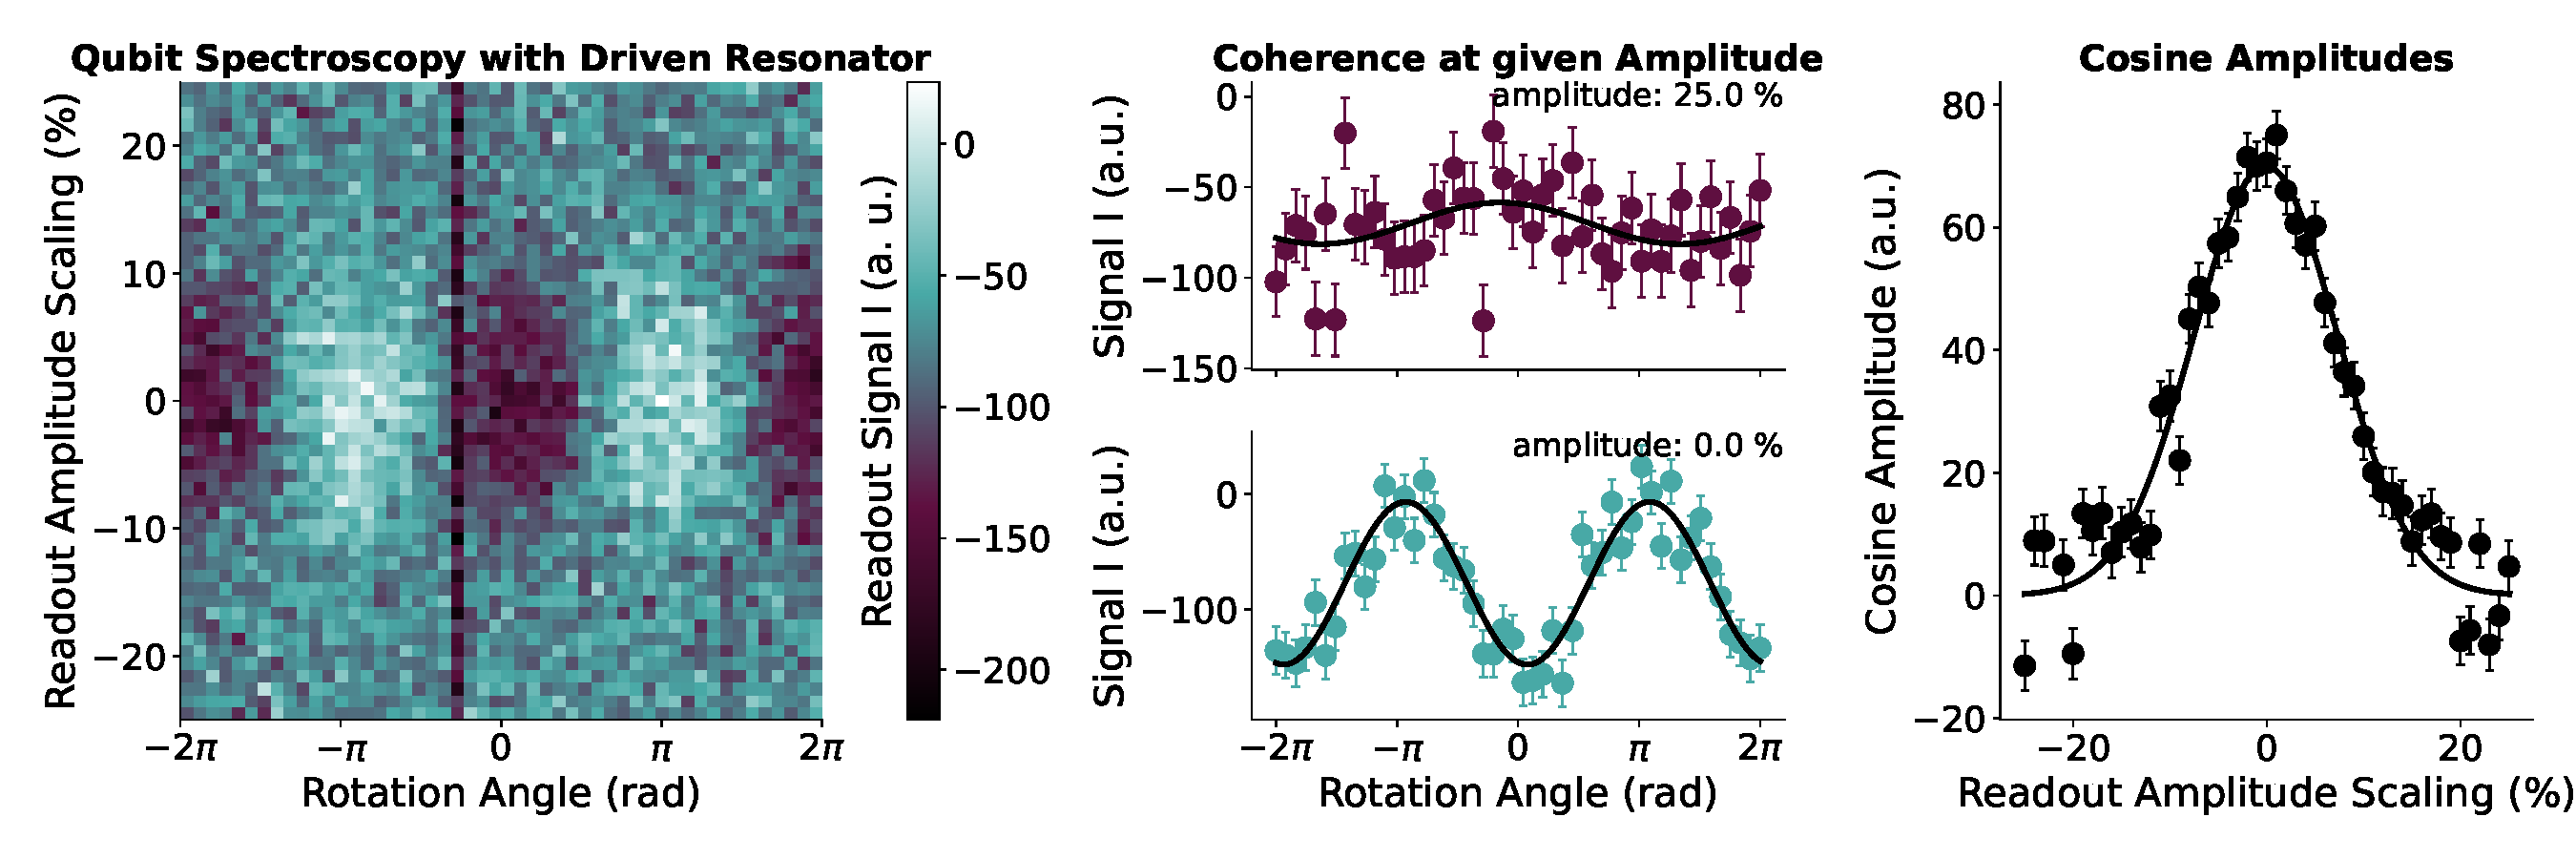
\includegraphics{Calibrations/Figures/dephasing_by_measurement.pdf}
    \caption{Results from the backaction experiment. The 2D scan is shown along with the cosine-way for amplitude $\epsilon = 0$ and $\epsilon = \epsilon_{max}$. Fitting the cosine function and plotting the amplitude as function of the readout amplitude gives the last figure, where they are are fitted by a gaussian distribution.}
    \label{fig:efficiency_dephasing_result}
\end{figure*}

\todo{Redo figure.}

\subsection{Calculating the Efficiency}
Combining the results from the last two experiments, we find the readout efficiency to be:
\begin{equation}
    \eta = \frac{a^2\sigma^2}{2} = (1.5 \pm ?) \% 
\end{equation}


\section{Calibration in Continuous Time}
To get significant statistics on some calibration, one sweep 1 or 2 values for the experiment and then repeat the experiment many times to get significant statistics. If one of the sweeping axis are duration, we could instead use a continous measurement scheme to get the same data. In this section, we look at calibration by continuous measurement to speed up calibration schemes. Further, we will discuss if measurement changes the physics significantly. 

\subsection{In-measurement T1 Calibration}
The times used for the $T_1$ calibration described in sec \ref{sec:calibration_t1} is mostly waiting to see if the qubit has decayed. If we instead were to do a measurement in the waiting time, we can split it up in chunks and do classification at many times in the same readout trace. If done right, this would allow us to completely remove the sweep axis and instead just repeat the experiment the appropriate amount to get the samples.

\begin{marginfigure}[-2cm]
    \centering
    \missingfigure{T1 circuit}
    \caption{Caption}
    \label{fig:inmeasurementt1circuit}
\end{marginfigure}

Performing the circuit described in figure \ref{fig:inmeasurementt1circuit} multiple times. We modulated the signal and course grained it in $10 \text{ ns}$ intervals to reduce data size. By doing $1 \text{ µs}$ summations and classifying\footnote{Classifcation schemes can be made by taking a subsample and drawing a thresh hold line with data from the first $1 \text{ µs}$ where the distribution most close resembles the initialization.} each individually, we can see the distribution of $\ket{0}$ and $\ket{1}$ over the entire readout duration. In an example with $50 \text{ µs}$ long readout the following distributions were found for qubit initialzied in the ground and first excited state respectively see figure \ref{fig:continous_calibration_decays}. 
\begin{figure}
    \centering
    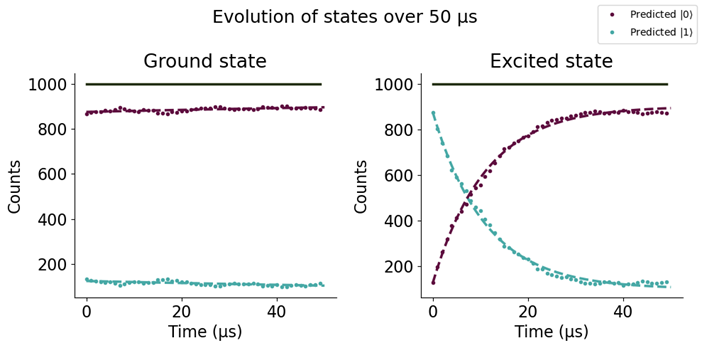
\includegraphics{Figs/calibrations/contiuous/decays.png}
    \caption{The dynamics of our qubit system from $50 \text{ µs}$ readout split into $1 \text{ µs}$ pieces which are all classified.}
    \label{fig:continous_calibration_decays}
\end{figure}
\begin{margintable}
    \centering
    \caption{Table of results from experiment}
    \begin{tabular}{c|cc}
        & Ground State & Excited state \\
        \hline
        $\rho(\infty)$&$0.951 \pm 0.254$&$0.099 \pm 0.004$ \\
        $\rho(0)$&$0.875 \pm 0.003$&$0.124 \pm 0.008$\\
        $T_1$ &$(159 \pm 615) \text{ µs}$&$(11.1 \pm 0.3)  \text{ µs}$\\
    \end{tabular}
    \label{tab:continous_calibration_decays_results}
\end{margintable}
    
The classification are the further fit by two curves with an exponential decay corresponding to the $\rho_{11}(t)$ and $\rho_{11}(t)$ from section \ref{sec:theory_t1}. To obtain the parameters displayed in table \ref{tab:continous_calibration_decays_results}. The most important detail is to extract the decay time $T_1 = (11.1\pm0.3) \text{ µs}$. This should be compared to a regular $T_1$ calibration giving $T_1^{reg} = 9.9 \pm 0.5 \text{ µs}$ done just before with $n$ samples and scanning the waiting time from $0 $ to $100 \text{ µs}$. \todo{Comment on results here}

Here, we also obtain the values for the steady state distributions $\rho(t \to \infty)$. In this limit, the system has reached equilibrium with the environment and the distribution is due to finite temperature. Comparing with the qubit frequency, we can calculate the temperature to be:
\begin{equation}
    \frac{p(\ket{1)}}{p(\ket{0})} = e^{(E_1 - E_0) / k_b \tau} \Leftarrow \tau = - \frac{\hbar \omega_{01}}{k_b} / \log\left(\frac{p(\ket{1)}}{p(\ket{0})} \right)  = 147.5 \text{ mK}
\end{equation}

\paragraph{Interleaved Experiment *}\todo{Do analysis} Since the $T_1$ can vary a lot over even small time periods, we also perform and interleaved version of the old and new experiment. This will also allow us to see if there is a different decay inside and outside of the measurement. In this experiment the previous one is carried out again but this time we will include a sweep over the waiting time before reading out for the same pulse length. We can now compare the in-measurement $T_1$ values from the fit within the same pulse with the ones across the waiting time. Given that we see a constant offset $T_1^{meas} = T_1^{wait} + \delta t$ this will show up in this experiment,

\begin{figure*}
    \centering
    \missingfigure{Analysis of interleaved experiment}
    \caption{Caption}
    \label{fig:enter-label}
\end{figure*}

Comments on results... 



\section{Overview of Device Parameters}
In this chapter, we have calibrated the necessary values of the qubit, resonator and system to be able to simulate the quantum system.


\begin{table}[h]
\centering
\caption{The outcome of calibrating the qubit with the methods presented in this chapter.}
\begin{tabular}{lr|rrr}
\hline
\textbf{Qubit}                &          & value & error & unit \\ \hline
Frequency                     & $f_{01}$ &  5.9823       &  0.0002  & Ghz  \\
Anharmonicity                 & $\alpha$ &  $-286.3$       &  0.3     & MHz  \\
Decay Time                    & $T_1$    &  2.94         &  0.08    & µs   \\
Dephasing Time                & $T_\phi$ &  2.39         &  0.12    & µs   \\ 
& & & & \\ \hline 

\textbf{Resonator}                &        & value      & error  & unit \\ \hline
Frequency                     & $f_{r}$    &  7.555135  & 9e-6?       & Ghz  \\
Disersive Shift               & $\chi$     &  745       &  9       & KHz \\
Decay rate                    & $\kappa$   &  2.7       & 0.3        & Mhz  \\
Mean Photon Number            & $\Bar{n}$  &  10.1      &  0.3   &  -  \\ 
& & & & \\ \hline 

\textbf{System}                &          & value & error & unit \\ \hline
Coupling                       & $g$      &  34.2         & 0.4    & Mhz  \\
Efficiency                     & $\eta$   &  1.5          &     & \% \\
Temperature                    & $\tau$   & 147.5         &      & mK 
\end{tabular}
\label{tab:qubit_calibration}
\end{table}